% ciac_ftfp.tex
%% for CIAC 2013 talk
%% and for phd defense (06/10/2013)
%%
\def\handout{0}
\def\notes{0}
\ifnum\handout=1
\documentclass[handout, hyperref, xcolor=dvipsnames]{beamer}
\usepackage{pgfpages}
\pgfpagesuselayout{4 on 1}[letterpaper,landscape,border shrink=4mm]
\setbeamertemplate{footline}[page number]
% use \setbeamertemplate{footline}[text line]{xxxx} if you want xxxx at bottom left of each slide
% use \setbeamertemplate{footline}[text line]{xxxx\hfill\thepage}
%  if you want xxxx at bottom left, page # at bottom right
\else
\documentclass[hyperref, xcolor=dvipsnames]{beamer}
\fi

\usepackage{amsmath, graphicx, tikz}
\usetikzlibrary{decorations.pathmorphing,arrows,positioning,shapes,shapes.multipart}

\title[FTFP]{Approximation Algorithms
  for the Fault-Tolerant Facility Placement Problem}
\author[lyan,marek]{Li Yan and Marek Chrobak}
\institute[UCR]{
  Computer Science\\
  University of California Riverside\\
}
\date{}
\usetheme{Warsaw}


%%%%%%%%%%%%%%%%%%%%%%%%%%%%%%%%%%%%%%%%%%%%%%%%%%%%%%%%%%

% non-math stuff

\newcommand{\myparagraph}[1]{{\medskip\noindent{\bf #1}}}
\newcommand{\emparagraph}[1]{{\medskip\noindent{\it #1}}}
\newcommand{\etal}{{\it et al.}}
\newcommand{\myif}{{\mbox{\rm\ if \ }}}
\newcommand{\mycase}[1]{\mbox{{\underline{Case #1}}:\/}}

\newcommand{\margincomment}[1]%
    {{%
      \marginpar{{\tiny\begin{minipage}{0.5in}
                       \begin{flushleft}
                          {#1}
                       \end{flushleft}
                       \end{minipage}
                }}
    }}


%%%%%%%%%%%%%%%%%%%%%%%%%%%%%%%%%%%%%%%%%%%%%%%%%%%%%%%%%%

% various letters

\newcommand{\hatc}{{\hat c}}
\newcommand{\hatC}{{\hat C}}
\newcommand{\hatr}{{\hat r}}
\newcommand{\hatx}{{\hat x}}
\newcommand{\haty}{{\hat y}}
\newcommand{\dotx}{{\dot x}}
\newcommand{\doty}{{\dot y}}
\newcommand{\dotr}{{\dot r}}
\newcommand{\boldx}{{\mathbf x}}

\newcommand{\doubledone}{{\bar 1}}
\newcommand{\doubledtwo}{{\bar 2}}
\newcommand{\barc}{{\bar c}}
\newcommand{\bart}{{\bar t}}

\newcommand{\barx}{{\bar x}}
\newcommand{\bary}{{\bar y}}
\newcommand{\barz}{{\bar z}}
\newcommand{\barr}{{\bar r}}
\newcommand{\barX}{{\bar X}}
\newcommand{\barY}{{\bar Y}}
\newcommand{\barZ}{{\bar Z}}
\newcommand{\bara}{{\bar a}}
\newcommand{\bard}{{\bar d}}
\newcommand{\barm}{{\bar m}}
\newcommand{\barA}{{\bar A}}
\newcommand{\barB}{{\bar B}}
\newcommand{\barC}{{\bar C}}
\newcommand{\barG}{{\bar G}}
\newcommand{\barE}{{\bar E}}
\newcommand{\barV}{{\bar V}}

\newcommand{\wbarC}{{\overline{C}}}
\newcommand{\wbarD}{{\overline{D}}}
\newcommand{\wbarN}{{\overline{N}}}
\newcommand{\wbarX}{{\overline{X}}}


\newcommand{\barbeta}{{\bar\beta}}
\newcommand{\bargamma}{{\bar\gamma}}
\newcommand{\apomega}{{\bar\omega}}

\newcommand{\bfr}{\boldsymbol{r}}
\newcommand{\bfv}{{\bf v}}
\newcommand{\bfx}{\boldsymbol{x}}
\newcommand{\bfy}{\boldsymbol{y}}
\newcommand{\bfz}{{\bf z}}
\newcommand{\bfQ}{{\bf Q}}
\newcommand{\bfR}{{\bf R}}
\newcommand{\bfS}{{\bf S}}
\newcommand{\bfT}{{\bf T}}
\newcommand{\bfV}{{\bf V}}
\newcommand{\bfone}{{\bf 1}}
\newcommand{\bfalpha}{\boldsymbol{\alpha}}
\newcommand{\bfbeta}{\boldsymbol{\beta}}

\newcommand{\calA}{{\cal A}}
\newcommand{\calB}{{\cal B}}
\newcommand{\calC}{{\cal C}}
\newcommand{\calD}{{\cal D}}
\newcommand{\calE}{{\cal E}}
\newcommand{\calG}{{\cal G}}
\newcommand{\calH}{{\cal H}}
\newcommand{\calJ}{{\cal J}}
\newcommand{\calK}{{\cal K}}
\newcommand{\calL}{{\cal L}}
\newcommand{\calM}{{\cal M}}
\newcommand{\calN}{{\cal N}}
\newcommand{\calS}{{\cal S}}
\newcommand{\calU}{{\cal U}}
\newcommand{\calX}{{\cal X}}
\newcommand{\calT}{{\cal T}}

\newcommand{\hatcalI}{{\hat{\cal I}}}
\newcommand{\barcalI}{{\bar{\cal I}}}
\newcommand{\dotcalI}{{\dot{\cal I}}}

\newcommand{\vecS}{{\bar S}}
\newcommand{\vecT}{{\bar T}}
\newcommand{\vecone}{{\bf 1}}
\newcommand{\tildec}{{\tilde c}}
\newcommand{\tilded}{{\tilde d}}
\newcommand{\tildeD}{{\tilde D}}
\newcommand{\tildeC}{{\widetilde C}}
\newcommand{\tildeZ}{{\tilde Z}}
\newcommand{\tilder}{{\widetilde r}}
\newcommand{\tildex}{{\widetilde x}}
\newcommand{\wtildeN}{{\widetilde N}}
\newcommand{\tildebfr}{\widetilde{\boldsymbol{r}}}
\newcommand{\tildebfx}{\widetilde{\boldsymbol{x}}}
\newcommand{\tildebfy}{\widetilde{\boldsymbol{y}}}

\newcommand{\barbfx}{\bar{\boldsymbol{x}}}
\newcommand{\barbfy}{\bar{\boldsymbol{y}}}
\newcommand{\hatbfx}{\hat{\boldsymbol{x}}}
\newcommand{\hatbfy}{\hat{\boldsymbol{y}}}
\newcommand{\dotbfx}{\dot{\boldsymbol{x}}}
\newcommand{\dotbfy}{\dot{\boldsymbol{y}}}

\newcommand{\wbarcalC}{{\overline{\calC}}}
\newcommand{\wbarcalD}{{\overline{\calD}}}
\newcommand{\eps}{{\epsilon}}

%%%%%%%%%%%%%%%%%%%%%%%%%%%%%%%%%%%%%%%%%%%%%%%%%%%%%%%%%%

\newcommand{\half}{{\mbox{$\frac{1}{2}$}}}
\newcommand{\threehalfs}{{\mbox{$\frac{3}{2}$}}}
\newcommand{\threefourths}{{\mbox{$\frac{3}{4}$}}}
\newcommand{\fivehalfs}{{\mbox{$\frac{5}{2}$}}}
\newcommand{\onethird}{{\mbox{$\frac{1}{3}$}}}
\newcommand{\twothirds}{{\mbox{$\frac{2}{3}$}}}
\newcommand{\fourthirds}{{\mbox{$\frac{4}{3}$}}}
\newcommand{\fivethirds}{{\mbox{$\frac{5}{3}$}}}
\newcommand{\fivefourths}{{\mbox{$\frac{5}{4}$}}}
\newcommand{\onefourth}{{\mbox{$\frac{1}{4}$}}}
\newcommand{\onefifth}{{\mbox{$\frac{1}{5}$}}}
\newcommand{\twofifths}{{\mbox{$\frac{2}{5}$}}}
\newcommand{\threefifths}{{\mbox{$\frac{3}{5}$}}}
\newcommand{\fourfifths}{{\mbox{$\frac{4}{5}$}}}
\newcommand{\ninefifths}{{\mbox{$\frac{9}{5}$}}}
\newcommand{\sevensixths}{{\mbox{$\frac{7}{6}$}}}
\newcommand{\oneeighth}{{\mbox{$\frac{1}{8}$}}}
\newcommand{\threeeighths}{{\mbox{$\frac{3}{8}$}}}
\newcommand{\fiveeighths}{{\mbox{$\frac{5}{8}$}}}
\newcommand{\seveneighths}{{\mbox{$\frac{7}{8}$}}}
\newcommand{\onetenth}{{\mbox{$\frac{1}{10}$}}}
\newcommand{\seventenths}{{\mbox{$\frac{7}{10}$}}}
\newcommand{\ninetenths}{{\mbox{$\frac{9}{10}$}}}
\newcommand{\twonineths}{{\mbox{$\frac{2}{9}$}}}
\newcommand{\fivenineths}{{\mbox{$\frac{5}{9}$}}}
\newcommand{\elevennineths}{{\mbox{$\frac{11}{9}$}}}
\newcommand{\threetwentieths}{{\mbox{$\frac{3}{20}$}}}
\newcommand{\twentyfivenineteenths}{{\mbox{$\frac{25}{19}$}}}

\newcommand{\sqrttwo}{\sqrt{2}}

%%%%%%%%%%%%%%%%%%%%%%%%%%%%%%%%%%%%%%%%%%%%%%%%%%%%%%%%%%

% various delimiters

\newcommand{\braced}[1]{{ \left\{ #1 \right\} }}
\newcommand{\angled}[1]{{ \left\langle #1 \right\rangle }}
\newcommand{\brackd}[1]{{ \left[ #1 \right] }}
\newcommand{\parend}[1]{{ \left( #1 \right) }}
\newcommand{\barred}[1]{{ \left| #1 \right| }}
\newcommand{\dbarred}[1]{{ \left\| #1 \right\| }}
\newcommand{\floor}[1]{{ \lfloor #1 \rfloor }}
\newcommand{\ceiling}[1]{{ \lceil #1 \rceil }}

%%%%%%%%%%%%%%%%%%%%%%%%%%%%%%%%%%%%%%%%%%%%%%%%%%%%%%%%%%

% some math symbols

\newcommand{\set}{\,{\leftarrow}\,}
\newcommand{\suchthat}{{\,:\,}}
\newcommand{\cost}{{\it cost}}
\newcommand{\yield}{{\it yield}}
\newcommand{\opt}{{\it opt}}

\newcommand{\algA}{{\bf A}}
\newcommand{\LHS}{{\rm LHS}}
\newcommand{\RHS}{{\rm RHS}}
\newcommand{\reals}{{\bf R}}
\newcommand{\posreals}{{\bf R}^+}

\newcommand{\assign}{{\,\leftarrow\,}}

\newcommand{\absvalue}[1]{{\barred{#1}}}
\newcommand{\posvalue}[1]{{\brackd{#1}^+}}

\newcommand{\NP}{{\mbox{\sf NP}}}
\newcommand{\PP}{{\mbox{\sf P}}}
\newcommand{\DTIME}{{\mbox{\sf DTIME}}}

\newcommand{\letbox}[1]{{\makebox[11pt]{{\small {$#1$}}}}}
\newcommand{\optstring}[1]{{ \frame{\;\raisebox{0pt}[12pt][5pt]{#1}\;} }}

\newcommand{\leftend}{{\diamond}}
\newcommand{\rightend}{{\diamond}}

%\newcommand{\argmin}{{\mbox{\rm argmin}}}
\DeclareMathOperator*{\argmin}{arg\,min}

\newcommand\litem[1]{\item{\bfseries #1\enspace}}
\newcommand{\ceil}[1] {\lceil #1 \rceil}
\newcommand{\naive}{na\"{\i}ve}
\newcommand{\LP}{\mbox{\rm LP}}
\newcommand{\OPT}{\mbox{\rm OPT}}
\newcommand{\ALG}{\mbox{\rm ALG}}
\newcommand{\LPR}[1]{{\mbox{\rm LPR#1}}}
\newcommand{\smallLPR}[1]{{\mbox{\tiny\rm LPR#1}}}
% algorithm names
\newcommand{\ESTA}{\mbox{\rm ESTA}} % 4approx
\newcommand{\EGUP}{\mbox{\rm EGUP}} % 3approx
\newcommand{\ECHS}{\mbox{\rm ECHS}} % 1.736
\newcommand{\EBGS}{\mbox{\rm EBGS}} % 1.575
\newcommand{\GUP}{\mbox{\rm GUP}}
\newcommand{\smallESTA}{\mbox{\tiny\rm ESTA}}
\newcommand{\smallEGUP}{\mbox{\tiny\rm EGUP}}
\newcommand{\smallECHS}{\mbox{\tiny\rm ECHS}}
\newcommand{\smallEBGS}{\mbox{\tiny\rm EBGS}}

\newcommand{\SOL}[1]{{{\mbox{\rm SOL}}_{#1}}}
\newcommand{\FTFP}{\mbox{\rm FTFP}}
\newcommand{\FTFL}{\mbox{\rm FTFL}}
\newcommand{\calI}{\mathcal{I}}
\newcommand{\avg}{{\mbox{\scriptsize\rm avg}}}

\newcommand{\dmax}{\text{dmax}}
\newcommand{\davg}{\text{davg}}
\newcommand{\favg}{f_{\text{avg}}}
\newcommand{\conn}{\text{conn}}
\newcommand{\cls}{\text{cls}}
\newcommand{\far}{\text{far}}

\newcommand{\sitesset}{\mathbb{F}}
\newcommand{\clientset}{\mathbb{C}}
\newcommand{\facilityset}{\overline{\sitesset}}
\newcommand{\demandset}{\overline{\clientset}}

%\newcommand{\dist}{{\mbox{dist}}}
\newcommand{\concost}{C^{\avg}}
\newcommand{\faccost}{F^{\avg}}
\newcommand{\tcc}{\mbox{\rm{tcc}}}
\newcommand{\clsdist}{C_{\cls}^{\avg}}
\newcommand{\fardist}{C_{\far}^{\avg}}
\newcommand{\clsmax}{C_{\cls}^{\max}}
\newcommand{\clsnb}{N_{\cls}}
\newcommand{\farnb}{N_{\far}}
\newcommand{\wbarclsnb}{\wbarN_{\cls}}
\newcommand{\wbarfarnb}{\wbarN_{\far}}
\newcommand{\wtildeclsnb}{\wtildeN_{\cls}}
\newcommand{\tcccls}{\mbox{\rm{tcc}}_{\cls}}
\newcommand{\dmaxcls}{\mbox{\rm{dmax}}_{\cls}}

\newcommand{\Exp}{\mbox{\rm Exp}}

\newcommand{\FacilityDistSort}{{\textsc{FacilityDistSort}}}
\newcommand{\NearestUnitChunk}{{\textsc{NearestUnitChunk}}}
\newcommand{\AugmentToUnit}{{\textsc{AugmentToUnit}}}
\newcommand{\connsum}{{\textrm{conn}}}

%%%%%%%%%%%%%%%%%%%%%%%%%%%%%%%%%%%%%%%%%%%%%%%%%%%%%%%%%%

% theorem and such

\newtheorem{theorem}{Theorem}
\newtheorem{definition}[theorem]{Definition}
\newtheorem{corollary}[theorem]{Corollary}
\newtheorem{lemma}[theorem]{Lemma}
\newtheorem{fact}[theorem]{Fact}
\newtheorem{claim}[theorem]{Claim}
\newtheorem{conjecture}[theorem]{Conjecture}
\newtheorem{observation}[theorem]{Observation}

%%%%%%%%%%%%%%%%%%%%%%%%%%%%%%%%%%%%%%%%%%%%%%%%%%%%%%%%%%

\newcommand{\ignore}[1]{}

\begin{document}

%%%
\begin{frame}
  \titlepage
\end{frame}

%%% outline
\begin{frame}
  \frametitle{Outline}
  \begin{enumerate}

  \item Problem Definition

  \item Related Work
    \begin{itemize}
    \item Uncapacitated Facility Location problem (UFL)
    \item Fault-tolerant Facility Location problem (FTFL)
    \item Fault-tolerant Facility Placement problem (FTFP)
    \end{itemize}

  \item Linear Program (LP) Formulation

  \item Demand Reduction

  \item Adaptive Partition

  \item LP-based Approximation Algorithms
      \begin{itemize}
        \item $3$-approximation
        \item $1.736$-approximation
        \item $1.575$-approximation
        \end{itemize}

  \item{Summary}
  \end{enumerate}
\end{frame}

%%% problem example
%%% instance with annotation
\begin{frame}
  \frametitle{Fault-tolerant Facility Placement Problem (FTFP)}
  \setbeamercovered{invisible}
  \begin{center}
  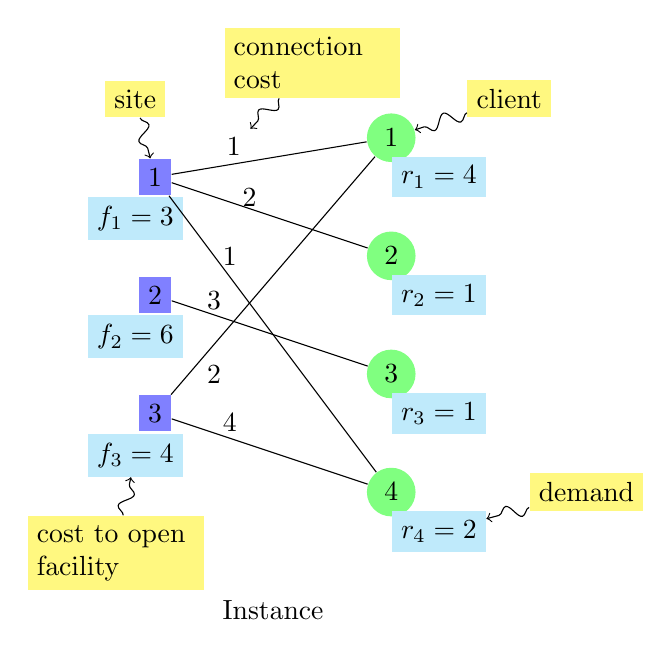
\begin{tikzpicture}[scale=0.5,decoration=snake]
    \node[fill=blue!50] (fac3) at (0,2) {$3$};
    \node[fill=blue!50] (fac2) at (0,5) {$2$};
    \node[fill=blue!50] (fac1) at (0,8) {$1$};

    \node[below,fill=cyan!25] (faclabel3) at (-.5,1.5) {$f_3=4$};
    \node[below,fill=cyan!25] (faclabel2) at (-.5,4.5) {$f_2=6$};
    \node[below,fill=cyan!25] (faclabel1) at (-.5,7.5) {$f_1=3$};

    \node[circle,fill=green!50] (client4) at (6,0) {$4$};
    \node[circle,fill=green!50] (client3) at (6,3) {$3$};
    \node[circle,fill=green!50] (client2) at (6,6) {$2$};
    \node[circle,fill=green!50] (client1) at (6,9) {$1$};

    \node[right,fill=cyan!25] (demand4) at (6,-1) {$r_4=2$};
    \node[right,fill=cyan!25] (demand3) at (6,2) {$r_3=1$};
    \node[right,fill=cyan!25] (demand2) at (6,5) {$r_2=1$};
    \node[right,fill=cyan!25] (demand1) at (6,8) {$r_1=4$};

    \foreach \from/\to in {fac3/client4,fac3/client1,fac2/client3,fac1/client4,fac1/client2,fac1/client1}
    \draw (\from)--(\to);

    % edge weight
    \node[above] (ew11) at (2,8.3) {$1$};
    \node[above] (ew12) at (2.4,7) {$2$};
    \node[above] (ew14) at (1.9,5.5) {$1$};
    \node[above] (ew23) at (1.5,4.4) {$3$};
    \node[above] (ew33) at (1.5,2.5) {$2$};
    \node[above] (ew34) at (1.9,1.3) {$4$};

    \node (label1) at (3,-3) {Instance};

    \pause
    % annotations
    \node[above,fill=yellow!50] (sites) at (-.5,9.5) {site}; 
    \draw[->,decorate] (sites) -- (fac1);
\pause
    \node[above,fill=yellow!50] (clients) at (9,9.5) {client};
    \draw[->,decorate] (clients) -- (client1);
\pause
    \node[right,fill=yellow!50] (demand) at (9.5,0) {demand};
    \draw[->,decorate] (demand) -- (demand4);
\pause
    \node[above,fill=yellow!50,text width=2cm] (fi) at (-1,-2.5) {cost to open facility};
    \draw[->,decorate] (fi) -- (faclabel3);
\pause
    \node[above,fill=yellow!50,text width=2cm] (edge) at (4,10) {connection cost};
    \draw[->,decorate] (edge) -- (ew11);
\pause
  \end{tikzpicture}
  \end{center}
\end{frame}

\begin{frame}
  \frametitle{Fault-tolerant Facility Placement Problem (FTFP)}

  \begin{center}
  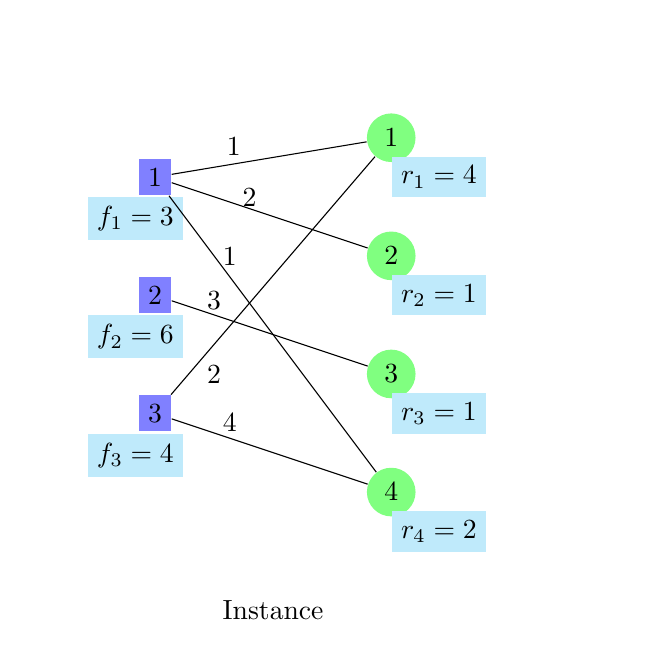
\begin{tikzpicture}[scale=0.5,decoration=snake]
    \node[fill=blue!50] (fac3) at (0,2) {$3$};
    \node[fill=blue!50] (fac2) at (0,5) {$2$};
    \node[fill=blue!50] (fac1) at (0,8) {$1$};

    \node[below,fill=cyan!25] (faclabel3) at (-.5,1.5) {$f_3=4$};
    \node[below,fill=cyan!25] (faclabel2) at (-.5,4.5) {$f_2=6$};
    \node[below,fill=cyan!25] (faclabel1) at (-.5,7.5) {$f_1=3$};

    \node[circle,fill=green!50] (client4) at (6,0) {$4$};
    \node[circle,fill=green!50] (client3) at (6,3) {$3$};
    \node[circle,fill=green!50] (client2) at (6,6) {$2$};
    \node[circle,fill=green!50] (client1) at (6,9) {$1$};

    \node[right,fill=cyan!25] (demand4) at (6,-1) {$r_4=2$};
    \node[right,fill=cyan!25] (demand3) at (6,2) {$r_3=1$};
    \node[right,fill=cyan!25] (demand2) at (6,5) {$r_2=1$};
    \node[right,fill=cyan!25] (demand1) at (6,8) {$r_1=4$};
    
    \foreach \from/\to in {fac3/client4,fac3/client1,fac2/client3,fac1/client4,fac1/client2,fac1/client1}
    \draw (\from)--(\to);

    % edge weight
    \node[above] (ew11) at (2,8.3) {$1$};
    \node[above] (ew12) at (2.4,7) {$2$};
    \node[above] (ew14) at (1.9,5.5) {$1$};
    \node[above] (ew23) at (1.5,4.4) {$3$};
    \node[above] (ew33) at (1.5,2.5) {$2$};
    \node[above] (ew34) at (1.9,1.3) {$4$};

    \node (label1) at (3,-3) {Instance};


    % remove annotations, use white, ugly solution
    \node[above,fill=white,color=white] (sites) at (-.5,9.5) {site}; 
    \draw[->,decorate,draw=none] (sites) -- (fac1);

    \node[above,fill=white,color=white] (clients) at (9,9.5) {client};
    \draw[->,decorate,draw=none] (clients) -- (client1);

    \node[right,fill=white,color=white] (demand) at (9.5,0) {demand};
    \draw[->,decorate,draw=none] (demand) -- (demand4);

    \node[above,fill=white,color=white,text width=2cm] (fi) at (-1,-2.5) {cost to open facility};
    \draw[->,decorate,draw=none] (fi) -- (faclabel3);

    \node[above,fill=white,color=white,text width=2cm] (edge) at (4,10) {connection cost};
    \draw[->,decorate,draw=none] (edge) -- (ew11);

  \end{tikzpicture}
  \end{center}
\end{frame}

%%% A feasible solution
\begin{frame}
  \frametitle{Feasible Integral Solution}

  \begin{minipage}{.4\linewidth}
  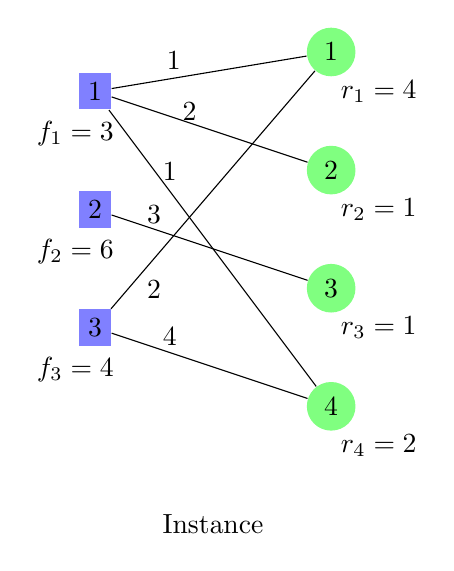
\begin{tikzpicture}[scale=0.5]
    \node[fill=blue!50] (fac3) at (0,2) {$3$};
    \node[fill=blue!50] (fac2) at (0,5) {$2$};
    \node[fill=blue!50] (fac1) at (0,8) {$1$};

    \node[below] (faclabel3) at (-.5,1.5) {$f_3=4$};
    \node[below] (faclabel2) at (-.5,4.5) {$f_2=6$};
    \node[below] (faclabel1) at (-.5,7.5) {$f_1=3$};

    \node[circle,fill=green!50] (client4) at (6,0) {$4$};
    \node[circle,fill=green!50] (client3) at (6,3) {$3$};
    \node[circle,fill=green!50] (client2) at (6,6) {$2$};
    \node[circle,fill=green!50] (client1) at (6,9) {$1$};

    \node[right] (demand4) at (6,-1) {$r_4=2$};
    \node[right] (demand3) at (6,2) {$r_3=1$};
    \node[right] (demand2) at (6,5) {$r_2=1$};
    \node[right] (demand1) at (6,8) {$r_1=4$};
    
    \foreach \from/\to in {fac3/client4,fac3/client1,fac2/client3,fac1/client4,fac1/client2,fac1/client1}
    \draw (\from)--(\to);

    % edge weight
    \node[above] (ew11) at (2,8.3) {$1$};
    \node[above] (ew12) at (2.4,7) {$2$};
    \node[above] (ew14) at (1.9,5.5) {$1$};
    \node[above] (ew23) at (1.5,4.4) {$3$};
    \node[above] (ew33) at (1.5,2.5) {$2$};
    \node[above] (ew34) at (1.9,1.3) {$4$};

    \node (label1) at (3,-3) {Instance};
  \end{tikzpicture}
  \end{minipage}
  \hspace{.5in}
  \begin{minipage}{.4\linewidth}
    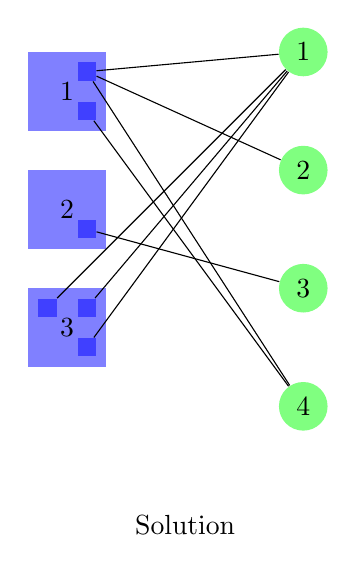
\begin{tikzpicture}[scale=0.5]
    \node[fill=blue!50,minimum size=1cm] (fac3) at (0,2) {$3$};
    \node[fill=blue!75,minimum size=.2cm] (fac33) at (.5,1.5) {};
    \node[fill=blue!75,minimum size=.2cm] (fac32) at (.5,2.5) {};
    \node[fill=blue!75,minimum size=.2cm] (fac31) at (-.5,2.5) {};

    \node[fill=blue!50,minimum size=1cm] (fac2) at (0,5) {$2$};
    \node[fill=blue!75,minimum size=.2cm] (fac21) at (.5,4.5) {};

    \node[fill=blue!50,minimum size=1cm] (fac1) at (0,8) {$1$};
    \node[fill=blue!75,minimum size=.2cm] (fac12) at (.5,7.5) {};
   \node[fill=blue!75,minimum size=.2cm] (fac11) at (.5,8.5) {};

    \node[circle,fill=green!50] (client4) at (6,0) {$4$};
    \node[circle,fill=green!50] (client3) at (6,3) {$3$};
    \node[circle,fill=green!50] (client2) at (6,6) {$2$};
    \node[circle,fill=green!50] (client1) at (6,9) {$1$};
    
    \foreach \from/\to in {fac31/client1,fac32/client1,fac33/client1,fac11/client1,fac11/client2,fac11/client4,fac21/client3,fac12/client4}
        \draw (\from)--(\to);
    
    \node (label1) at (3,-3) {Solution};
  \end{tikzpicture}
  \end{minipage}
  \vspace{.1in}

  Cost is $2f_1 + f_2 + 3f_3 + d_{11} + d_{12} + 2d_{14} +
  d_{23} + 3d_{31} = 38$
\end{frame}

\begin{frame}
  \frametitle{Optimal Integral Solution}
  \begin{minipage}{.4\linewidth}
  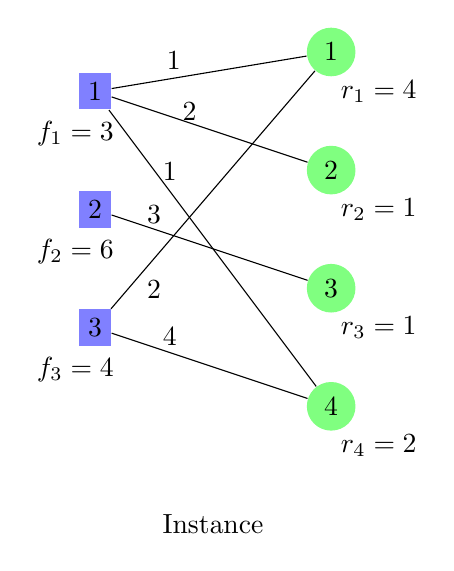
\begin{tikzpicture}[scale=0.5]
    \node[fill=blue!50] (fac3) at (0,2) {$3$};
    \node[fill=blue!50] (fac2) at (0,5) {$2$};
    \node[fill=blue!50] (fac1) at (0,8) {$1$};

    \node[below] (faclabel3) at (-.5,1.5) {$f_3=4$};
    \node[below] (faclabel2) at (-.5,4.5) {$f_2=6$};
    \node[below] (faclabel1) at (-.5,7.5) {$f_1=3$};

    \node[circle,fill=green!50] (client4) at (6,0) {$4$};
    \node[circle,fill=green!50] (client3) at (6,3) {$3$};
    \node[circle,fill=green!50] (client2) at (6,6) {$2$};
    \node[circle,fill=green!50] (client1) at (6,9) {$1$};

    \node[right] (demand4) at (6,-1) {$r_4=2$};
    \node[right] (demand3) at (6,2) {$r_3=1$};
    \node[right] (demand2) at (6,5) {$r_2=1$};
    \node[right] (demand1) at (6,8) {$r_1=4$};
    
    \foreach \from/\to in {fac3/client4,fac3/client1,fac2/client3,fac1/client4,fac1/client2,fac1/client1}
    \draw (\from)--(\to);

    % edge weight
    \node[above] (ew11) at (2,8.3) {$1$};
    \node[above] (ew12) at (2.4,7) {$2$};
    \node[above] (ew14) at (1.9,5.5) {$1$};
    \node[above] (ew23) at (1.5,4.4) {$3$};
    \node[above] (ew33) at (1.5,2.5) {$2$};
    \node[above] (ew34) at (1.9,1.3) {$4$};

    \node (label1) at (3,-3) {Instance};
  \end{tikzpicture}    
  \end{minipage}
  \hspace{.5in}
  \begin{minipage}{.4\linewidth}
    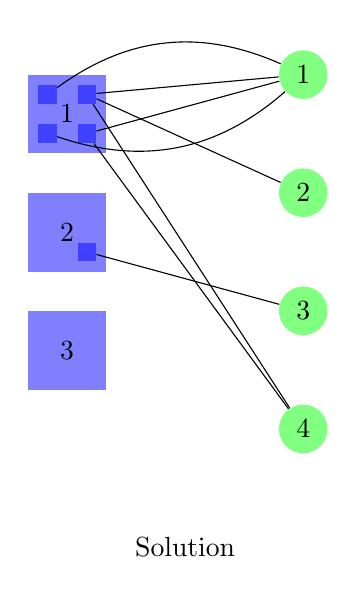
\begin{tikzpicture}[scale=0.5]
    \node[fill=blue!50,minimum size=1cm] (fac3) at (0,2) {$3$};

    \node[fill=blue!50,minimum size=1cm] (fac2) at (0,5) {$2$};
    \node[fill=blue!75,minimum size=.2cm] (fac21) at (.5,4.5) {};

    \node[fill=blue!50,minimum size=1cm] (fac1) at (0,8) {$1$};
    \node[fill=blue!75,minimum size=.2cm] (fac14) at (-.5,7.5) {};
    \node[fill=blue!75,minimum size=.2cm] (fac13) at (-.5,8.5) {};
    \node[fill=blue!75,minimum size=.2cm] (fac12) at (.5,7.5) {};
    \node[fill=blue!75,minimum size=.2cm] (fac11) at (.5,8.5) {};

    \node[circle,fill=green!50] (client4) at (6,0) {$4$};
    \node[circle,fill=green!50] (client3) at (6,3) {$3$};
    \node[circle,fill=green!50] (client2) at (6,6) {$2$};
    \node[circle,fill=green!50] (client1) at (6,9) {$1$};
    
    \foreach \from/\to in {fac11/client1,fac12/client1,fac11/client2,fac11/client4,fac12/client4,fac21/client3}
        \draw (\from)--(\to);

    \draw[bend left] (fac13) to node (ew13) {} (client1);
    \draw[bend right] (fac14) to node (ew14) {} (client1);
    \node (label1) at (3,-3) {Solution};
  \end{tikzpicture}
  \end{minipage}
  \vspace{.1in}

  Cost is $4f_1 + 1f_2 + 0f_3 + 4d_{11} + d_{12} + 2d_{14} +
  d_{23} = 29$
\end{frame}
%%% problem definition
\begin{frame}
  \frametitle{Fault-Tolerant Facility Placement Problem (FTFP)}
  Given
  \begin{itemize}
  \item $\sitesset$, a set of sites (facility places)
  \item $\clientset$, a set of clients with demands
  \item $r_j$, demand for client $j$
  \item $f_i$, cost to open one facility at site $i$
  \item $d_{ij}$, cost to connect one demand from client $j$ to
    facility at site $i$
  \end{itemize}
  Assume Distances form a metric

  Objective
  \begin{itemize}
  \item open facilities at each site
  \item connect clients to facilities
  \item minimize the total cost = (facility cost) + (connection cost)
  \end{itemize}

\end{frame}

%%% related problem
\begin{frame}
  \frametitle{Related Problems}
  \begin{center}
  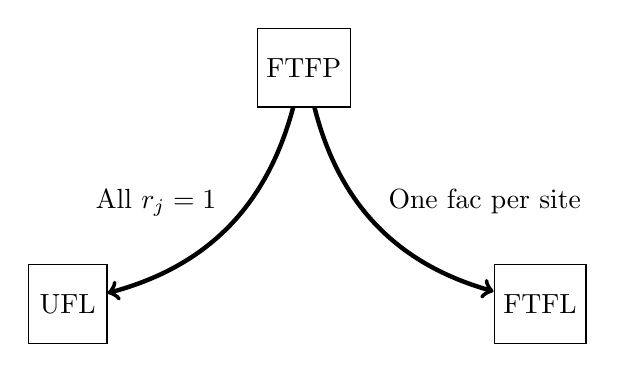
\begin{tikzpicture}[auto]
    \node[rectangle, draw, minimum size=1cm] (ftfp) at (0,0) {FTFP};
    \node[rectangle, draw, minimum size=1cm] (ufl) at (-3,-3) {UFL};
    \node[rectangle, draw, minimum size=1cm] (ftfl) at (3,-3) {FTFL};
    
    \draw[->,ultra thick, bend left] (ftfp) to node [swap] {All $r_j=1$} (ufl);
    \draw[->,ultra thick, bend right] (ftfp) to node {One fac per site} (ftfl);
  \end{tikzpicture}
  \end{center}
  \begin{itemize}
  \item Uncapacitated Facility Location problem (UFL),
    all clients have unit demand.
  \item Fault-tolerant Facility Location problem (FTFL),
    each site can have at most one facility.
  \end{itemize}
\end{frame}

%%% UFL example
\begin{frame}
  \frametitle{Uncapacitated Facility Location Problem (UFL)}
  All demands are 1, each site can open only one facility
  \begin{minipage}{.45\linewidth}
  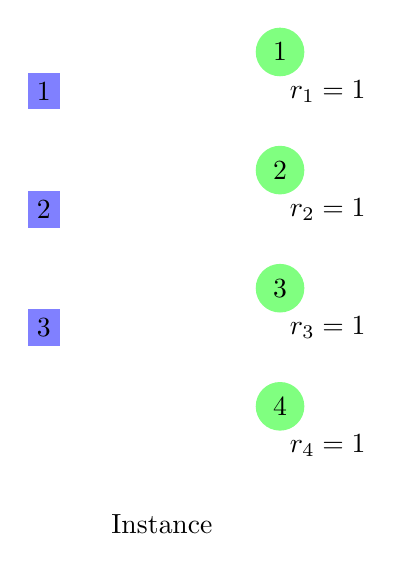
\begin{tikzpicture}[scale=0.5]
    \node[fill=blue!50,minimum size=.2cm] (fac3) at (0,2) {$3$};
    \node[fill=blue!50,minimum size=.2cm] (fac2) at (0,5) {$2$};
    \node[fill=blue!50,minimum size=.2cm] (fac1) at (0,8) {$1$};

    \node[circle,fill=green!50,minimum size=.2cm] (client4) at (6,0) {$4$};
    \node[circle,fill=green!50,minimum size=.2cm] (client3) at (6,3) {$3$};
    \node[circle,fill=green!50,minimum size=.2cm] (client2) at (6,6) {$2$};
    \node[circle,fill=green!50,minimum size=.2cm] (client1) at (6,9) {$1$};

    \node[right] (demand1) at (6,-1) {$r_4=1$};
    \node[right] (demand2) at (6,2) {$r_3=1$};
    \node[right] (demand3) at (6,5) {$r_2=1$};
    \node[right] (demand4) at (6,8) {$r_1=1$};
    
    \node (label1) at (3,-3) {Instance};
  \end{tikzpicture}
  \end{minipage}
  \begin{minipage}{.45\linewidth}
  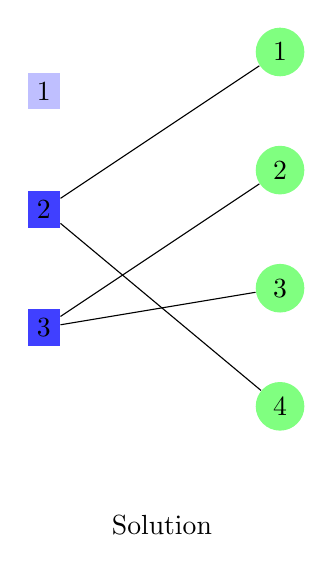
\begin{tikzpicture}[scale=0.5]
    \node[fill=blue!75,minimum size=.2cm] (fac3) at (0,2) {$3$};
    \node[fill=blue!75,minimum size=.2cm] (fac2) at (0,5) {$2$};
    \node[fill=blue!25,minimum size=.2cm] (fac1) at (0,8) {$1$};

    \node[circle,fill=green!50,minimum size=.2cm] (client4) at (6,0) {$4$};
    \node[circle,fill=green!50,minimum size=.2cm] (client3) at (6,3) {$3$};
    \node[circle,fill=green!50,minimum size=.2cm] (client2) at (6,6) {$2$};
    \node[circle,fill=green!50,minimum size=.2cm] (client1) at (6,9) {$1$};

    \foreach \from/\to in {fac2/client1,fac2/client4,fac3/client2,fac3/client3}
        \draw (\from)--(\to);

    \node (label2) at (3,-3) {Solution};
  \end{tikzpicture}
  \end{minipage}

\end{frame}

%%% FTFL example
\begin{frame}
  \frametitle{Fault-tolerant Facility Location Problem (FTFL)}
  Demands may be more than 1, each site can open only one facility

  \begin{minipage}{.45\linewidth}
  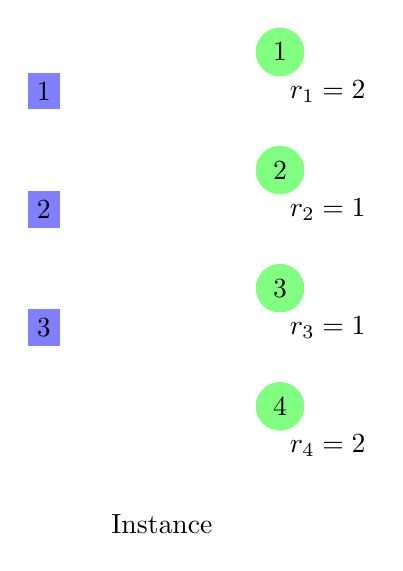
\begin{tikzpicture}[scale=0.5]
    \node[fill=blue!50,minimum size=.2cm] (fac3) at (0,2) {$3$};
    \node[fill=blue!50,minimum size=.2cm] (fac2) at (0,5) {$2$};
    \node[fill=blue!50,minimum size=.2cm] (fac1) at (0,8) {$1$};

    \node[circle,fill=green!50,minimum size=.2cm] (client1) at (6,0) {$4$};
    \node[circle,fill=green!50,minimum size=.2cm] (client2) at (6,3) {$3$};
    \node[circle,fill=green!50,minimum size=.2cm] (client3) at (6,6) {$2$};
    \node[circle,fill=green!50,minimum size=.2cm] (client4) at (6,9) {$1$};

    \node[right] (demand1) at (6,-1) {$r_4=2$};
    \node[right] (demand2) at (6,2) {$r_3=1$};
    \node[right] (demand3) at (6,5) {$r_2=1$};
    \node[right] (demand4) at (6,8) {$r_1=2$};

    \node (label1) at (3,-3) {Instance};    
  \end{tikzpicture}
  \end{minipage}
  \begin{minipage}{.45\linewidth}
  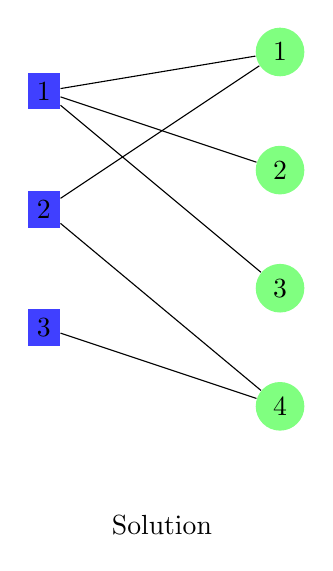
\begin{tikzpicture}[scale=0.5]
    \node[fill=blue!75,minimum size=.2cm] (fac3) at (0,2) {$3$};
    \node[fill=blue!75,minimum size=.2cm] (fac2) at (0,5) {$2$};
    \node[fill=blue!75,minimum size=.2cm] (fac1) at (0,8) {$1$};

    \node[circle,fill=green!50,minimum size=.2cm] (client4) at (6,0) {$4$};
    \node[circle,fill=green!50,minimum size=.2cm] (client3) at (6,3) {$3$};
    \node[circle,fill=green!50,minimum size=.2cm] (client2) at (6,6) {$2$};
    \node[circle,fill=green!50,minimum size=.2cm] (client1) at (6,9) {$1$};
    
    \foreach \from/\to in {fac1/client1,fac1/client2,fac1/client3,fac2/client1,fac2/client4,fac3/client4}
        \draw (\from)--(\to);

        \node (label2) at (3,-3) {Solution};
  \end{tikzpicture}
  \end{minipage}

\end{frame}

%%% FTFP example
\begin{frame}
  \frametitle{Fault-tolerant Facility Placement Problem (FTFP)}
  Demands may be more than 1, each site can open multiple facilities

  \begin{minipage}{.45\linewidth}
  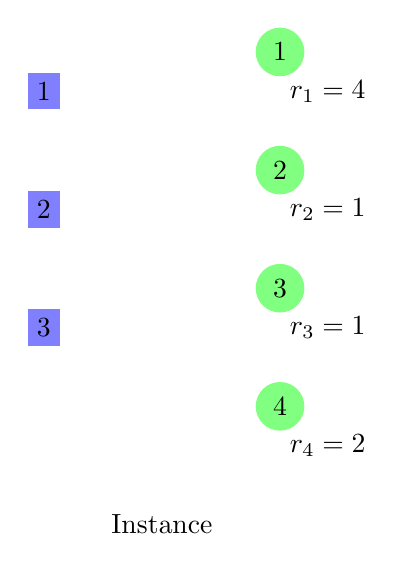
\begin{tikzpicture}[scale=0.5]
    \node[fill=blue!50] (fac3) at (0,2) {$3$};
    \node[fill=blue!50] (fac2) at (0,5) {$2$};
    \node[fill=blue!50] (fac1) at (0,8) {$1$};

    \node[circle,fill=green!50] (client4) at (6,0) {$4$};
    \node[circle,fill=green!50] (client3) at (6,3) {$3$};
    \node[circle,fill=green!50] (client2) at (6,6) {$2$};
    \node[circle,fill=green!50] (client1) at (6,9) {$1$};

    \node[right] (demand4) at (6,-1) {$r_4=2$};
    \node[right] (demand3) at (6,2) {$r_3=1$};
    \node[right] (demand2) at (6,5) {$r_2=1$};
    \node[right] (demand1) at (6,8) {$r_1=4$};
    
    \node (label1) at (3,-3) {Instance};
  \end{tikzpicture}
  
  \end{minipage}
  \begin{minipage}{.45\linewidth}
    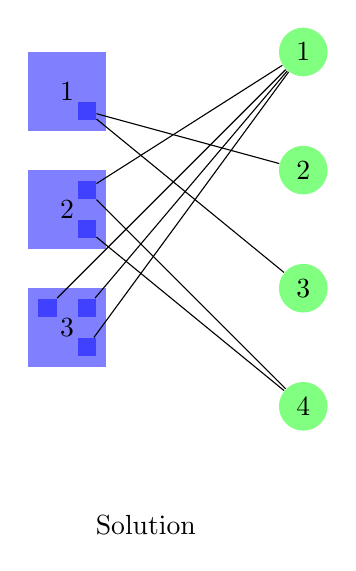
\begin{tikzpicture}[scale=0.5]
    \node[fill=blue!50,minimum size=1cm] (fac3) at (0,2) {$3$};
    \node[fill=blue!75,minimum size=.2cm] (fac31) at (.5,1.5) {};
    \node[fill=blue!75,minimum size=.2cm] (fac32) at (.5,2.5) {};
    \node[fill=blue!75,minimum size=.2cm] (fac33) at (-.5,2.5) {};

    \node[fill=blue!50,minimum size=1cm] (fac2) at (0,5) {$2$};
    \node[fill=blue!75,minimum size=.2cm] (fac21) at (.5,4.5) {};
    \node[fill=blue!75,minimum size=.2cm] (fac22) at (.5,5.5) {};

    \node[fill=blue!50,minimum size=1cm] (fac1) at (0,8) {$1$};
    \node[fill=blue!75,minimum size=.2cm] (fac11) at (.5,7.5) {};

    \node[circle,fill=green!50] (client4) at (6,0) {$4$};
    \node[circle,fill=green!50] (client3) at (6,3) {$3$};
    \node[circle,fill=green!50] (client2) at (6,6) {$2$};
    \node[circle,fill=green!50] (client1) at (6,9) {$1$};
    
    \foreach \from/\to in {fac31/client1,fac32/client1,fac33/client1,fac22/client1,fac21/client4,fac22/client4,fac11/client3,fac11/client2}
        \draw (\from)--(\to);

    \node (label2) at (2,-3) {Solution};
  \end{tikzpicture}
\end{minipage}
\end{frame}


%%% related work
\begin{frame}
  \frametitle{Related Work on UFL}

  Approximation algorithms for UFL

  \vspace{.3in}
  \begin{tabular}{| c | c | c | c |}
    \hline
    Shmoys, Tardos and Aardal & 1997 & 3.16 & LP-rounding\\
    Chudak & 1998 & 1.736 & LP-rounding\\
    Sviridenko & 2002 & 1.58 & LP-rounding\\
    \hline
    Jain and Vazirani & 2001 & 3 & primal-dual\\
    Jain {\etal} & 2002 & 1.61 & greedy\\
    Mahdian {\etal} & 2002 & 1.52 & greedy\\
    \hline
    Byrka & 2007 & 1.5 & hybrid\\
    Li & 2011 & 1.488 & hybrid (best result)\\
    \hline
  \end{tabular}
  \vspace{.3in}

  \begin{tabular}{| c | c | c | c |}
    \hline
    lower bound (inapproximability) & Guha and Khuller & 1998 & 1.463\\
    \hline
  \end{tabular}
\end{frame}

\begin{frame}
  \frametitle{Related Work on FTFL}

    Approximation algorithms for FTFL

    \vspace{.3in}
    \begin{tabular}{| c | c | c | c |}
      \hline
      Jain and Vazirani & 2000 & $3\ln \max_j r_j$ & primal-dual\\
      \hline
      Guha {\etal} & 2001 & 4 & LP-rounding\\
      Byrka {\etal} & 2010 & 1.7245 & LP-rounding\\
      \hline
    \end{tabular}
    \vspace{.5in}

  \textbf{Remark:} No combinatorial algorithm for FTFL with
  approximation ratio better than $O(\log n)$ is known.
\end{frame}


%%% our results
\begin{frame}
  \frametitle{Our Result for FTFP}

  \begin{itemize}
  \item Main result: 1.575-approximation LP-rounding algorithm
  \item Our ratio for FTFP matches the best known LP-based
    approximation ratio for UFL
  \item Generalize known LP-rounding algorithms for UFL to algorithms for FTFP
  \end{itemize}
\end{frame}


%%% LP-formulation
\begin{frame}
  \frametitle{LP Formulation for FTFP}
  \begin{itemize}
  \item $y_i$   number of facilities open at site $i\in \sitesset$
  \item $x_{ij}$ number of connections from client $j\in
    \clientset$ to site $i \in \sitesset$
  \end{itemize}
  %%%%%%%%%%% 
  \begin{alignat}{3}
    \textrm{minimize}\quad \sum f_iy_i &+ \sum d_{ij}x_{ij}&
    \\ \notag
    \textrm{subject to}\quad y_i - x_{ij} &\geq 0  & &\forall i,j
    \\ \notag
    \sum x_{ij} &\geq r_j & &\forall j
    \\ \notag
    x_{ij} \geq 0, y_i &\geq 0 & &\forall i,j
    \\ \notag
  \end{alignat}
  %%%%%%%%%%%%
  \begin{alignat}{3}
  \text{(Dual)}\quad  \textrm{maximize}\quad \sum r_j\, \alpha_j&
    \\ \notag
    \textrm{subject to} \quad 
      \sum \beta_{ij} &\leq f_i  &\quad\quad			&\forall i
    \\ \notag
    \alpha_{j} - \beta_{ij} 	&\leq  d_{ij}       &                 & \forall i,j
    \\ \notag
    \alpha_j \geq 0, \beta_{ij} &\geq 0           &            & \forall i,j
  \end{alignat}
  %%%%%%%%%%%
\end{frame}

%%% Techniques
\begin{frame}
  \frametitle{Techniques}
  \begin{itemize}
  \item Demand Reduction
    \begin{itemize}
    \item Using optimal LP solution to reduce all $r_j$ to small value
    \item Ensure partitioning and rounding in polynomial time
    \end{itemize}
    
  \item Adaptive Partition
    \begin{itemize}
    \item Split sites into facilities and clients into unit demands
    \item Split associated fractional values
    \item Allow rounding generalized from that for UFL
    \end{itemize}
  \end{itemize}
\end{frame}


%%% figure for demand reduction
\begin{frame}
  \frametitle{Algorithm for FTFP}
  \begin{center}
  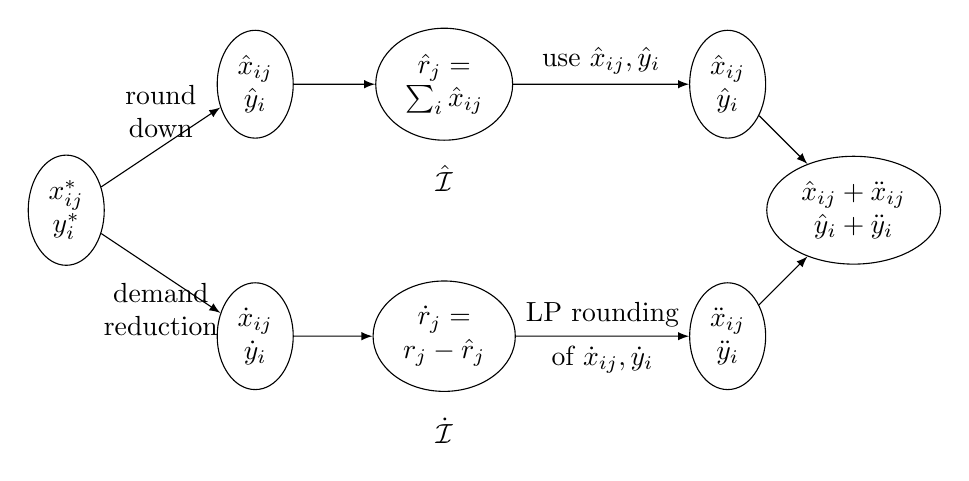
\begin{tikzpicture}[auto,scale=.8,every text node part/.style={align=center}]
    \node[draw,ellipse] (lpsoln) at (0,0) {$x_{ij}^\ast$\\ $y_{i}^\ast$};
    \node[draw,ellipse] (intpart) at (3,2) {$\hatx_{ij}$\\ $\haty_{i}$};
    \node[draw,ellipse] (fracpart) at (3,-2) {$\dotx_{ij}$\\ $\doty_{i}$};

    \node[draw,ellipse] (intinst) at (6,2) {$\hatr_j =$ \\ $\sum_{i} \hatx_{ij}$};
    \node (intlabel) at (6,.5) {$\hat\calI$};
    \node[draw,ellipse] (fracinst) at (6,-2) {$\dotr_j = $\\ $r_j - \hatr_j$};
    \node (fraclabel) at (6,-3.5) {$\dot\calI$};

    \node[draw, ellipse] (intsoln) at (10.5,2) {$\hatx_{ij}$ \\ $\haty_i$};
%    \node (intsoln1) at (9,0) {Soln for $\hat \calI$};
    \node[draw, ellipse] (fracsoln) at (10.5,-2) {$\ddot x_{ij}$ \\ $\ddot y_i$};
%    \node (fracsoln1) at (9,-4) {Soln for $\dot \calI$};
    \node[draw, ellipse] (soln) at (12.5,0) {$\hatx_{ij} + \ddot x_{ij}$ \\ $\haty_i + \ddot y_i$};
%    \node (soln1) at (12,-2) {Soln for $\calI$};

    \draw[->,>=latex] (lpsoln) to node[above] (trim) {round\\ down} (intpart);
    \draw[->,>=latex] (lpsoln) to node[below] (rem) {demand\\ reduction} (fracpart);
    \draw[->,>=latex] (intpart) to (intinst);
    \draw[->,>=latex] (fracpart) to (fracinst);
    \draw[->,>=latex] (intinst) to node (edge) {use $\hatx_{ij}, \haty_i$} (intsoln);
    \draw[->,>=latex] (fracinst) to node (edge) {LP rounding} node[swap] (edge) {of $\dotx_{ij}, \doty_{i}$} (fracsoln);
    \draw[->,>=latex] (intsoln) to (soln);
    \draw[->,>=latex] (fracsoln) to (soln);    

  \end{tikzpicture}
  \end{center}
\end{frame}

%%% demand reduction
\begin{frame}
  \frametitle{Demand Reduction}

  \begin{itemize}
  \item Solving LP for $(\bfx^\ast, \bfy^\ast)$.
  \item $\hat\bfx, \hat\bfy = $ round down $\bfx^\ast, \bfy^\ast$
  \item $\dot\bfx, \dot\bfy = $ remaining fractional
  \item $\hat r_j = \sum_{i}\hat x_{ij}$ for $\hat\calI$, $\dot r_j = r_j - \hat r_j$ for $\dot\calI$
  \item $\hat\bfx, \hat\bfy$ feasible and optimal for $\hat\calI$
  \item $\dot\bfx, \dot\bfy$ feasible and optimal for $\dot\calI$
  \end{itemize}
\end{frame}




%%%%%%%%%%%%%%%%%%%%%%%%%%%%%%%%%%%%%%%%%%%%%
%%% old partitioning slides
%%%%%%%%%%%%%%%%%%%%%%%%%%%%%%%%%%%%%%%%%%%%%
%%\begin{frame}
%%  \frametitle{Adaptive Partition}
%%  \begin{itemize}
%%  \item Begin with a fractional complete solution $(\bfx,\bfy)$.
%%  \item In the partitioned solution,
%%    \begin{itemize}
%%    \item Each site $i$ has facilities $\mu$.
%%    \item Each client $j$ has $r_j$ demand points $\nu$.
%%    \item Each facility $\mu$ has fractional opening $\bary_{\mu}$.
%%    \item Each demand point connects to each facility with value
%%      $\barx_{\mu\nu}$.
%%    \end{itemize}
%%    \item The partitioned solution $(\barbfx,\barbfy)$ satisfies a
%%      number of properties.
%%      \begin{itemize}
%%      \item $y_i^\ast$ distributed among facilities at site $i$,
%%      \item $x_{ij}^\ast$ distributed among sibling demands of client
%%        $j$,
%%      \item $\barx_{\mu\nu} = \bary_{\mu}$ or $0$ (completeness),
%%      \item Each demand $\nu$ is assigned to a primary demand $\kappa$
%%        with a low cost.
%%      \end{itemize}
%%  \end{itemize}
%%\end{frame}
%%
%%\begin{frame}
%%  \frametitle{Animation of Partition}
%%
%%  Two phases
%%  \begin{itemize}
%%  \item Phase 1, the partitioning phase, define demands and allocate facilities.
%%  \item Phase 2, the augmenting phase, allocate additional facilities
%%    to make total connection value unit.
%%  \end{itemize}
%%\end{frame}
%%
%%\begin{frame}
%%  \frametitle{Phase 1, Step 1} 
%%  \setbeamercovered{invisible}
%%
%%  For each client $j$ with residual demand $\barr_j > 0$, arrange
%%  neighboring facilities from near to far. The nearest few with total
%%  connection value $1$ defines $\wbarN_1(j)$.
%%  
%%  \begin{center}
%%  \begin{tikzpicture}
%%    \node (label1) at (-2,5) {$\wtildeN_1(j)$};
%%    \node (label2) at (4,4) {$\wtildeN(j)$};
%%
%%    \draw (0,0) ellipse (3cm and .8cm);
%%    \draw (0,2) ellipse (3cm and .8cm);
%%    \draw (0,4) ellipse (3cm and .8cm);
%%
%%
%%    %% squares, facilities
%%    \draw[fill=blue!50] (-1.5,0) rectangle (-2,.4);
%%    \draw[fill=blue!50] (-.8,-.1) rectangle (-1.3,.3);
%%    \draw[fill=blue!50] (-1.3,-.2) rectangle (-1.8,-.6);
%%
%%    \draw[fill=blue!50] (0,0) rectangle (.5,.4);
%%    \draw[fill=blue!50] (1.3,-.2) rectangle (1.8,-.6);
%%         
%%    \draw[fill=blue!50] (-1.5,2) rectangle (-2,2.4);
%%    \draw[fill=blue!50] (-.8,1.9) rectangle (-1.3,2.3);
%%    \draw[fill=blue!50] (-1.3,1.8) rectangle (-1.8,1.4);
%%
%%    \draw[fill=blue!50] (.2,1.8) rectangle (.7,1.4);
%%    \draw[fill=blue!50] (1,1.8) rectangle (1.5,1.4);
%%
%%    \draw[fill=blue!50] (-1.5,4) rectangle (-2,4.4);
%%    \draw[fill=blue!50] (-.8,3.9) rectangle (-1.3,4.3);
%%    \draw[fill=blue!50] (-1.3,3.8) rectangle (-1.8,3.4);
%%
%%    \draw[fill=blue!50] (0,3.4) rectangle (.5,3.8);
%%    \draw[fill=blue!50] (.3,4) rectangle (.8,4.4);
%%    \draw[fill=blue!50] (2,3.6) rectangle (2.5,4);
%%
%%    \pause
%%    \draw[style=dashed] (-.5,-1) -- (-.5,5);
%%  \end{tikzpicture}
%%  \end{center}
%%\end{frame}
%%
%%\begin{frame}
%%  \frametitle{Phase 1, Step 2} 
%%
%%  Select client $p$ such that the sum of the average distance to
%%  $\wtildeN_1(p)$ and $\alpha_p^\ast$ is minimized. Now we have two
%%  cases to proceed.
%%
%%  \begin{itemize}
%%  \item Case 1: $\wtildeN_1(p)$ is disjoint from every exisiting
%%    $\wbarN(\kappa)$.
%%    \begin{center}
%%    \begin{tikzpicture}
%%    \draw (0,0) ellipse (2cm and 1cm);
%%    \draw (5,0) ellipse (2cm and 1cm);
%%    \node (text1) at (0,-1.5) {$\wtildeN_1(p)$};
%%    \node (text2) at (5,-1.5) {$\wbarN(\kappa)$};
%%    \end{tikzpicture}
%%    \end{center}
%%  \item Case 2: $\wtildeN_1(p)$ overlaps with some $\wbarN(\kappa)$.
%%  \end{itemize}
%%  \begin{center}
%%    \begin{tikzpicture}
%%    \draw (3,0) ellipse (2cm and 1cm);
%%    \draw (5.5,0) ellipse (2cm and 1cm);
%%    \node (text1) at (3,-1.5) {$\wtildeN_1(p)$};
%%    \node (text2) at (5.5,-1.5) {$\wbarN(\kappa)$};
%%    \end{tikzpicture}
%%    \end{center}
%%\end{frame}
%%
%%%%% make a new primary
%%\begin{frame}
%%  \frametitle{Phase 1, Step 2 (Cont. Case 1)}
%%  \begin{center}
%%  \begin{tikzpicture}
%%    \draw[fill=yellow!50] (0,0) ellipse (3.3cm and 2.3cm);
%%    \node[right] at (0,-3) {$\wtildeN(p)$};
%%    
%%    \draw[fill=yellow!50] (-1,0) ellipse (1cm and 2cm);
%%    \node[above] at (-1,-1) {$\wtildeN_1(p)$};
%%    
%%    \draw[fill=blue!50] (-1,1.2) rectangle (-.5,1.7);
%%    \draw[fill=blue!50] (-1.5,.4) rectangle (-1,.9);
%%    \draw[fill=blue!50] (-1,-.2) rectangle (-.5,.3);
%%
%%    \draw (5,0) ellipse (1cm and 2cm);
%%    \node[right] at (6,0) {$\wbarN(\nu)$};
%%  \end{tikzpicture}
%%  \end{center}
%%\end{frame}
%%
%%\begin{frame}
%%  \frametitle{Phase 1, Step 2 (Cont. Case 1)}
%%
%%  All facilities in $\wtildeN_1(p)$ moved to $\wbarN(\nu)$.
%%  
%%  \vspace{1cm}
%%  \begin{center}
%%  \begin{tikzpicture}
%%    \draw[fill=yellow!50] (0,0) ellipse (3.3cm and 2.3cm);
%%    \node[right] at (0,-3) {$\wtildeN(p)$};
%%    
%%    \draw[fill=white] (-1,0) ellipse (1cm and 2cm);
%%    
%%    \draw[fill=yellow!50] (5,0) ellipse (1cm and 2cm);
%%    \node[right] at (6,0) {$\wbarN(\nu)$};
%%
%%    \draw[fill=blue!50] (5,1.2) rectangle (5.5,1.7);
%%    \draw[fill=blue!50] (4.5,.4) rectangle (5,.9);
%%    \draw[fill=blue!50] (5,-.2) rectangle (5.5,.3);
%%
%%  \end{tikzpicture}
%%  \end{center}
%%\end{frame}
%%
%%%%% intersect with a primary
%%\begin{frame}
%%  \frametitle{Phase 1, Step 2 (Cont. Case 2)}
%%
%%  Move all overlapping facilities in $\wtildeN(p) \cap
%%  \wbarN(\kappa)$ into $\wbarN(\nu)$.
%%
%%  \vspace{.5cm}
%%  \begin{center}
%%  \begin{tikzpicture}
%%  \draw[fill=green!50] (1,1) ellipse (1.5cm and 2.5cm);
%%  \node (client) at (-1,0) {$\wtildeN(p)$};
%%
%%  \draw[fill=yellow!50] (1.2,1.5) ellipse (.7cm and 1.4cm);
%%  \node (prefix) at (1.3,.7) {$\wbarN_1(p)$};
%%
%%  \draw (1,3) ellipse (1cm and 2cm);
%%  \node (primary) at (-.5,4) {$\wbarN(\kappa)$};
%%
%%  \draw (7,1) ellipse (2cm and 1cm);
%%  \node (demand) at (7,-.5) {$\wbarN(\nu)$};
%%
%%  %% fac
%%  \draw[fill=blue!50] (1.2,2) rectangle (1.7,2.5);
%%  \draw[fill=blue!50] (.4,2.8) rectangle (.9,3.3);
%%  \draw[fill=blue!50] (.6,1.5) rectangle (1.1,2);
%%
%%  \draw [->,>=latex] (1.7,2) -- (7,1);
%%  \draw [->,>=latex] (.9,3) -- (7,1.5);
%%  \draw [->,>=latex] (.9,1.5) -- (7,.5);
%%  \end{tikzpicture}
%%  \end{center}
%%\end{frame}
%%
%%\begin{frame}
%%  \frametitle{Phase 2}
%%
%%  Add facilities from $\wtildeN(j)$ to $\wbarN(\nu)$ until total
%%  connection value is $1$.
%%
%%  \vspace{1cm}
%%  \begin{center}
%%  \begin{tikzpicture}
%%    \draw (0,0) ellipse (3cm and 2cm);
%%    \node (label1) at (0,-2.5) {$\wtildeN(j)$};
%%
%%    \draw (5,0) ellipse (1cm and 2cm);
%%    \node (label2) at (5,-2.5) {$\wbarN(\nu)$};
%%
%%    \draw[fill=blue!50] (-2.5,0) rectangle (-2,.5);
%%    \draw[fill=blue!50] (-2,-1) rectangle (-1.5,-.5);
%%    \draw[fill=blue!50] (-1,.5) rectangle (-.5,1);
%%    \draw[fill=blue!50] (2,0) rectangle (2.5,.5);
%%
%%    \draw[fill=blue!50] (5,1) rectangle (5.5,1.5);
%%    \draw[fill=blue!50] (5,-1.5) rectangle (5.5,-1);
%%
%%    \draw [->,>=latex] (2.5,.3) -- (5,0);
%%  \end{tikzpicture}
%%  \end{center}
%%
%%\end{frame}

\begin{frame}
  \frametitle{Adaptive Partition}
  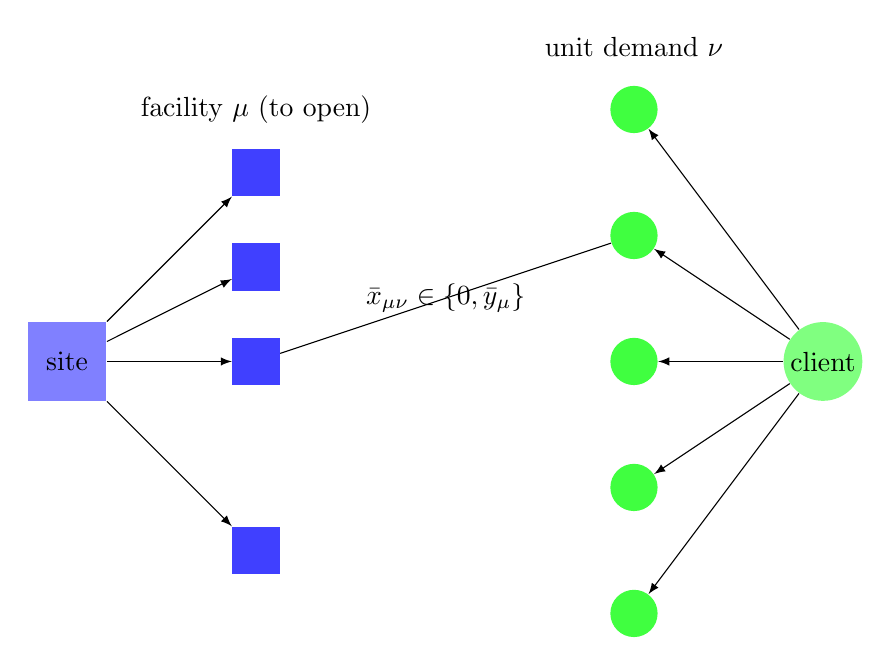
\begin{tikzpicture}[scale=.8]
    % site to facility
    \node[fill=blue!50,minimum size=1cm] (site) at (0,0) {};
    \node[fill=blue!75,minimum size=.6cm] (fac1) at (3,3) {};
    \node[fill=blue!75,minimum size=.6cm] (fac2) at (3,1.5) {};
    \node[fill=blue!75,minimum size=.6cm] (fac3) at (3,0) {};
    \node[fill=blue!75,minimum size=.6cm] (fack) at (3,-3) {};

    \foreach \from in {site}
    \foreach \to in {fac1,fac2,fac3,fack}
    \draw[->,>=latex] (\from) -- (\to);

    \node (sitelabel) at (0,0) {site};
    \node (faclabel) at (3,4) {facility $\mu$ (to open)};

    % client to demand
    \node[circle, fill=green!50, minimum size=1cm] (client) at (12,0) {};
    \node[circle, fill=green!75, minimum size=.6cm] (demand1) at (9,4) {};
    \node[circle, fill=green!75, minimum size=.6cm] (demand2) at (9,2) {};
    \node[circle, fill=green!75, minimum size=.6cm] (demand3) at (9,0) {};
    \node[circle, fill=green!75, minimum size=.6cm] (demand4) at (9,-2) {};
    \node[circle, fill=green!75, minimum size=.6cm] (demandk) at (9,-4) {};
    \foreach \from in {client}
    \foreach \to in {demand1, demand2, demand3, demand4, demandk}
    \draw[->,>=latex] (\from) -- (\to);

    \node (clientlabel) at (12,0) {client};
    \node (demandlabel) at (9,5) {unit demand $\nu$};

    % xval
    \draw (fac3) to node (xval) {$\barx_{\mu\nu} \in \{0, \bary_{\mu}\}$} (demand2);
  \end{tikzpicture}
\end{frame}

%%% neigbhorhood
\begin{frame}
  \frametitle{Neighborhood}
  \begin{center}
  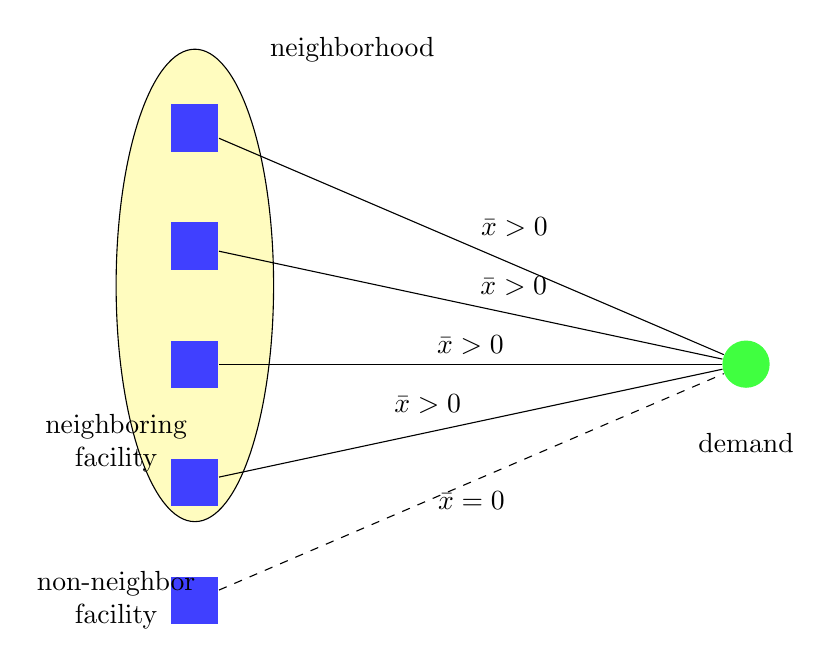
\begin{tikzpicture}[auto,every text node part/.style={align=center}]
    \draw[fill=yellow!25] (3,1) ellipse (1cm and 3cm);

    \node[fill=blue!75,minimum size=.6cm] (fac1) at (3,3) {};
    \node[fill=blue!75,minimum size=.6cm] (fac2) at (3,1.5) {};
    \node[fill=blue!75,minimum size=.6cm] (fac3) at (3,0) {};
    \node[fill=blue!75,minimum size=.6cm] (fac4) at (3,-1.5) {};
    \node[fill=blue!75,minimum size=.6cm] (fac5) at (3,-3) {};

    \node[circle,fill=green!75,minimum size=.6cm] (demand) at (10,0){};

    \foreach \from in {fac1,fac2,fac3,fac4}
    \foreach \to in {demand}
    \draw (\from) to node (edgelabel) {$\barx > 0$} (\to);

    \draw[dashed] (fac5) to node[below] (zerolabel) {$\barx = 0$} (demand);

    \node (neighborlabel) at (5,4) {neighborhood};
    \node (faclabel) at (2,-1) {neighboring \\ facility};
    \node (otherlabel) at (2,-3) {non-neighbor \\ facility};
    \node (demandlabel) at (10,-1) {demand};
  \end{tikzpicture}
  \end{center}
\end{frame}


\begin{frame}
  \frametitle{Partition Properties}
  \begin{itemize}
  \item 
  \end{itemize}
\end{frame}
%%% partition example
\begin{frame}
  \frametitle{An Example of Partition}

  \begin{minipage}{.45\linewidth}
  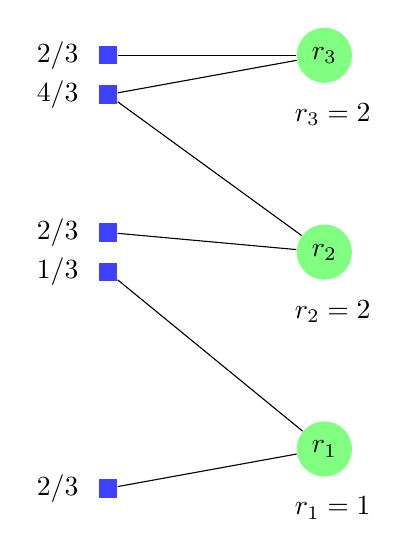
\begin{tikzpicture}[scale=0.5]
    \node[fill=blue!75,minimum size=.2cm] (fac11) at (.5,1) {};
    \node[left] (faclabel22) at (0,1) {$2/3$};

    \node[fill=blue!75,minimum size=.2cm] (fac21) at (.5,6.5) {};
    \node[fill=blue!75,minimum size=.2cm] (fac22) at (.5,7.5) {};

    % label
    \node[left] (faclabel21) at (0,6.5) {$1/3$};
    \node[left] (faclabel22) at (0,7.5) {$2/3$};

    \node[fill=blue!75,minimum size=.2cm] (fac31) at (.5,11) {};
    \node[fill=blue!75,minimum size=.2cm] (fac32) at (.5,12) {};

    % label
    \node[left] (faclabel31) at (0,11) {$4/3$};
    \node[left] (faclabel32) at (0,12) {$2/3$};

    \node[circle,fill=green!50] (client1) at (6,2) {$r_1$};
    \node[circle,fill=green!50] (client2) at (6,7) {$r_2$};
    \node[circle,fill=green!50] (client3) at (6,12) {$r_3$};

    \node[right] (demand1) at (5,.5) {$r_1=1$};
    \node[right] (demand2) at (5,5.5) {$r_2=2$};
    \node[right] (demand3) at (5,10.5) {$r_3=2$};
  
    \foreach \from/\to in {fac11/client1,fac21/client1,fac22/client2,fac31/client2,fac31/client3,fac32/client3}
    \draw (\from)--(\to);

  \end{tikzpicture}
  
  Before Partition
  \end{minipage}
  \begin{minipage}{.45\linewidth}
    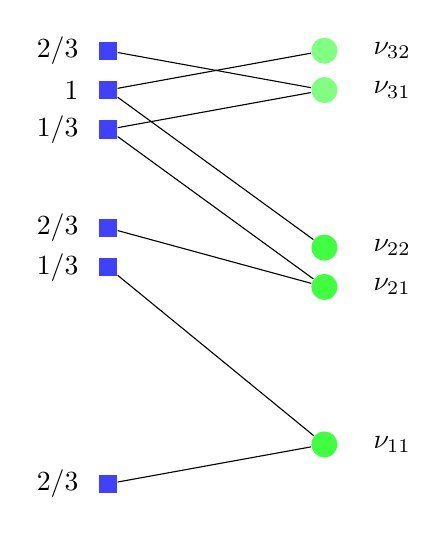
\begin{tikzpicture}[scale=0.5]
    \node[fill=blue!75,minimum size=.2cm] (fac11) at (.5,1) {};
    \node[left] (faclabel22) at (0,1) {$2/3$};

    \node[fill=blue!75,minimum size=.2cm] (fac21) at (.5,6.5) {};
    \node[fill=blue!75,minimum size=.2cm] (fac22) at (.5,7.5) {};

    % label
    \node[left] (faclabel21) at (0,6.5) {$1/3$};
    \node[left] (faclabel22) at (0,7.5) {$2/3$};

    \node[fill=blue!75,minimum size=.2cm] (fac31) at (.5,10) {};
    \node[fill=blue!75,minimum size=.2cm] (fac32) at (.5,11) {};
    \node[fill=blue!75,minimum size=.2cm] (fac33) at (.5,12) {};

    % label
    \node[left] (faclabel31) at (0,10) {$1/3$};
    \node[left] (faclabel32) at (0,11) {$1$};
    \node[left] (faclabel33) at (0,12) {$2/3$};

    \node[circle,fill=green!75,minimum size=.2cm] (client11) at (6,2) {};
    \node[circle,fill=green!75,minimum size=.2cm] (client21) at (6,6) {};
    \node[circle,fill=green!75,minimum size=.2cm] (client22) at (6,7) {};
    \node[circle,fill=green!50,minimum size=.2cm] (client31) at (6,11) {};
    \node[circle,fill=green!50,minimum size=.2cm] (client32) at (6,12) {};


    \node[right] (demand11) at (7,2) {$\nu_{11}$};
    \node[right] (demand21) at (7,6) {$\nu_{21}$};
    \node[right] (demand22) at (7,7) {$\nu_{22}$};
    \node[right] (demand31) at (7,11) {$\nu_{31}$};
    \node[right] (demand32) at (7,12) {$\nu_{32}$};

    \foreach \from/\to in {fac11/client11,fac21/client11,fac22/client21,fac31/client21,fac32/client22,fac31/client31,fac33/client31,fac32/client32}
    \draw (\from)--(\to);
  \end{tikzpicture}
      
  After Partition
\end{minipage}
\end{frame}

%%%
\begin{frame}
  \frametitle{Properties of Partition}
  Properties
  \begin{itemize}
  \item Each demand $\nu$ assigned to a primary demand $\kappa$ with
    overlapping $\wbarN(\nu)$ and $\wbarN(\kappa)$.
  \item For sibling demands $\nu_1$ and $\nu_2$, $\wbarN(\nu_1) \cup
    \wbarN(\kappa_1)$ is disjoint from $\wbarN(\nu_2) \cup
    \wbarN(\kappa_2)$.
  \item For a certain cost specified by the approximation algorithm,
    $\kappa$ always have a lower cost compared to the assigned $\nu$.
  \end{itemize}

  Implication
  \begin{itemize}
  \item The fractional solution can be rounded to a fault-tolerant
    integral solution.
  \item The cost of the integral solution can be approximated.
  \end{itemize}
\end{frame}

%%% 3-approx
\begin{frame}
  \frametitle{A $3$-approximation Algorithm}
  Given $(\barbfx,\barbfy)$, rounded by
  \begin{itemize}
  \item For each primary $\kappa$, choose facility $\mu$ in
    neighborhood with probability $\bary_{\mu}$.
  \item For each non-primary $\nu$, connects to $\phi(\kappa)$, the
    facility chosen in the primary's neighborhood.
  \end{itemize}

  The rounded solution satisfies fault-tolerant requirement.

  The rounded solution has cost at most $3\LP^\ast$.
  \begin{itemize}
  \item Facility cost is at most $F^\ast$.
  \item For each demand $\nu$, connection cost is at most $\sum_{\mu
      \in \wbarN(\nu)} d_{\mu\nu} \barx_{\mu\nu} + 2\alpha_{\nu}^\ast$.
  \end{itemize}
\end{frame}

%%% 1+2/e approx
\begin{frame}
  \frametitle{A $1.736$-approximation Algorithm} 

  \begin{itemize}
  \item Change in rounding: 
    \begin{itemize}
    \item For facilities $\mu$ not in any $\wbarN(\kappa)$, round
      indedendently.
    \item each non-primary $\nu$ uses nearest neighboring facility if
      one is open, else use $\phi(\kappa)$.
    \end{itemize}
  \item
  The expected connection cost for $\nu$ now reduced to $\sum_{\mu
      \in \wbarN(\nu)} d_{\mu\nu} \barx_{\mu\nu} + 2/e\cdot
    \alpha_{\nu}^\ast$.
  \end{itemize}
\end{frame}

%%% 1.575-approx
\begin{frame}
  \frametitle{Refined Partition for $1.575$-approximation}
  Properties
  \begin{itemize}
  \item $\wbarN(\nu)$ consists of $\wbarclsnb(\nu)$ and
    $\wbarfarnb(\nu)$ and they are disjoint.
  \item $\wbarclsnb(\nu)$ overlaps with $\wbarclsnb(\kappa)$.
  \item For siblings $\nu_1, \nu_2$, $\wbarclsnb(\kappa_1) \cup
    \wbarN(\nu_1)$ disjoint from $\wbarclsnb(\kappa_2) \cup
    \wbarN(\nu_2)$.
  \item cost of $\kappa$ is smaller than cost of $\nu$.
  \end{itemize}
\end{frame}

\begin{frame}
  \frametitle{Construction of Partition}
  \begin{itemize}
  \item Allocation.
  \item Augmentation.
  \end{itemize}
\end{frame}

\begin{frame}
  \frametitle{$1.575$-approximation}

  \begin{itemize}
  \item Use Byrka's rounding.
  \item $\nu$ uses only facilities in $\wbarN(\nu) \cup
    \wbarclsnb(\kappa)$. Thus no two sibling conflict.
  \item Cost analysis is similar to Byrka's for UFL.
  \end{itemize}
\end{frame}

\begin{frame}
  \Huge{The End.}
\end{frame}

%%%%%%%%%%%%%%%%%%%%%%%%%%%%%%%%%%%%%%%%%%%%%%%%%%%%%%%%%%
%%%%%%%%%%%%%%%%%%%%%%%%%%%%%%%%%%%%%%%%%%%%%%%%%%%%%%%%%%
%% legacy slides
%%%%%%%%%%%%%%%%%%%%%%%%%%%%%%%%%%%%%%%%%%%%%%%%%%%%%%%%%%


%%%
%%\begin{frame}
%%  \frametitle{UFL Background: Cont.}
%%
%%  The Shmoys, Tardos and Ardal's Algorithm (STA97)
%%  \begin{itemize}
%%  \item Start with optimal fractional solution $(\bfx^\ast,\bfy^\ast)$
%%  \item If all $N(j)$ disjoint, then easy.
%%  \item To bound $F^A$, need neighborhood of chosen clients be disjoint.
%%  \item To bound $C^A$, need non-primary clients having a fail-over connection.
%%  \end{itemize}
%%
%%  \begin{itemize}
%%  \item The greedy clustering: iteratively find the best client and assign some other clients to it.
%%  \item Estimate $\max_{i\in N(j)} d_{ij}$, either cut the neighborhood $N(j)$ or use dual solution.
%%  \end{itemize}
%%\end{frame}
%%
%%\begin{frame}
%%  \frametitle{UFL background: Cont.}
%%  The Clustering Structure
%%  \begin{tikzpicture}
%%    % fac group
%%    \draw[style=dashed] (0,0) ellipse (.5 and 1);
%%    \draw[fill=blue!50] (-.15,-.7) rectangle (.1,-.45);
%%    \draw[fill=blue!50] (-.15,-.2) rectangle (.1,.05);
%%    \draw[fill=blue!50] (-.15,.3) rectangle (.1,.55);
%%
%%    \draw[style=dashed] (0,2.5) ellipse (.5 and 1);
%%    \draw[fill=blue!50] (-.15,2) rectangle (.1,2.25);
%%    \draw[fill=blue!50] (-.15,2.5) rectangle (.1,2.75);
%%
%%    \draw[style=dashed] (0,6) ellipse (.5 and 1);
%%    \draw[fill=blue!50] (-.15,5.1) rectangle (.1,5.35);
%%    \draw[fill=blue!50] (-.15,5.6) rectangle (.1,5.85);
%%    \draw[fill=blue!50] (-.15,6.1) rectangle (.1,6.35);
%%    \draw[fill=blue!50] (-.15,6.6) rectangle (.1,6.85);
%%
%%    % client group
%%    \draw[style=dashed] (6,0) ellipse (4 and 1);
%%    \draw[fill=yellow!50] (3,0) circle (.25);
%%    \draw[fill=green!50] (5,0) circle (.25);
%%    \draw[fill=green!50] (6,0) circle (.25);
%%    \draw[fill=green!50] (7,0) circle (.25);
%%    \draw[fill=green!50] (9,0) circle (.25);
%%
%%    \draw[style=dashed] (6,2.5) ellipse (4 and 1);
%%    \draw[fill=yellow!50] (3,2.5) circle (.25);
%%    \draw[fill=green!50] (5,2.5) circle (.25);
%%    \draw[fill=green!50] (6,2.5) circle (.25);
%%    \draw[fill=green!50] (7,2.5) circle (.25);
%%    \draw[fill=green!50] (9,2.5) circle (.25);
%%
%%    \draw[style=dashed] (6,6) ellipse (4 and 1);
%%    \draw[fill=yellow!50] (3,6) circle (.25);
%%    \draw[fill=green!50] (5,6) circle (.25);
%%    \draw[fill=green!50] (6,6) circle (.25);
%%    \draw[fill=green!50] (7,6) circle (.25);
%%    \draw[fill=green!50] (9,6) circle (.25);
%%
%%    % lines
%%    \path[draw] (2.75,6) -- (.25,6.9);
%%    \path[draw] (2.75,6) -- (.25,5.1);
%%
%%    \path[draw] (2.75,2.5) -- (.25,3.4);
%%    \path[draw] (2.75,2.5) -- (.25,1.6);
%%
%%    \path[draw] (2.75,0) -- (.25,.9);
%%    \path[draw] (2.75,0) -- (.25,-.9);
%%  \end{tikzpicture}
%%\end{frame}
%%%%%
%%\begin{frame}
%%  \frametitle{UFL Background: End.}
%%
%%  Chudak, Svi, Byrka and Li's improvement
%%  \begin{itemize}
%%  \item Chudak: randomized rounding, estimate on the expected connection cost
%%  \item Sviridenko: use a concave function to upper bound distance and to guide rounding
%%  \item Byrka: boost facility opening probability and use $N_{\cls}(j)$ for overlapping
%%  \item Li: find the right distribution for probability boost
%%  \end{itemize}
%%\end{frame}
%%
%%%%%
%%\begin{frame}
%%  \frametitle{Contribution: Approximation Algorithms for FTFP}
%%
%%  \begin{itemize}
%%  \item LP-rounding Algorithms
%%    \begin{itemize}
%%    \item Demand Reduction
%%    \item Adaptive Partition
%%    \item 1.575 Approximation
%%    \end{itemize}
%%  \item Combinatorial Algorithms
%%    \begin{itemize}
%%    \item $O((\log R / \log\log R)^2)$ approximation
%%    \item Analysis of Greedy
%%    \end{itemize}
%%  \end{itemize}
%%\end{frame}
%%
%%%%%
%%\begin{frame}
%%  \frametitle{LP for the FTFP Problem}
%%  \begin{itemize}
%%  \item $y_i$ represent the number of facilities built at site $i$.
%%  \item $x_{ij}$ represent the number of connections from client $j$
%%    to facilities at site $i$.
%%  \end{itemize}
%%  %%%%%%%%%%% 
%%  \begin{alignat}{3}
%%    \notag
%%    \textrm{minimize}\quad \textstyle{\sum_{i\in \sitesset}}f_iy_i &+ \textstyle{\sum_{i\in \sitesset, j\in \clientset}}d_{ij}x_{ij}&
%%    \\ \notag
%%    \textrm{subject to}\quad y_i - x_{ij} &\geq 0  & &\forall i\in \sitesset, j\in \clientset 
%%    \\ \notag
%%    \textstyle{\sum_{i\in \sitesset} x_{ij}} &\geq r_j & &\forall j\in \clientset
%%    \\ \notag
%%    x_{ij} \geq 0, y_i &\geq 0 & &\forall i\in \sitesset, j\in \clientset 
%%    \\ \notag
%%  \end{alignat}
%%  %%%%%%%%%%%%
%%  \begin{alignat}{3}
%%    \notag
%%    \textrm{maximize}\quad \textstyle{\sum_{j\in \clientset}} r_j\alpha_j&
%%    \\ \notag
%%    \textrm{subject to} \quad \textstyle{
%%      \sum_{j\in \clientset}\beta_{ij}} &\leq f_i  &\quad\quad			&\forall i \in \sitesset  
%%    \\ \notag
%%    \alpha_{j} - \beta_{ij} 	&\leq  d_{ij}       &                 & \forall i\in \sitesset, j\in \clientset 
%%    \\ \notag
%%    \alpha_j \geq 0, \beta_{ij} &\geq 0           &            & \forall i\in \sitesset, j\in \clientset
%%  \end{alignat}
%%  %%%%%%%%%%%
%%\end{frame}
%%
%%%%%
%%\begin{frame}
%%  \frametitle{Demand Reduction} Given an FTFP instance $\calI$, we can
%%  reduce it to an instance such that $R=\max_{j}r_j$ is bounded by
%%  $|\sitesset|$.
%%
%%  \begin{itemize}
%%    \item $\hatx_{ij} = \floor{x_{ij}^\ast}, \haty_{i} = \floor{y_i^\ast}$
%%    \item $\dotx_{ij} = x_{ij}^\ast - \hatx_{ij}, \doty_{i} = y_i^\ast
%%      - \haty_{i}$
%%    \item $\hatr_j = \sum_{i\in\sitesset} \hatx_{ij}$ for instance $\hat \calI$
%%    \item $\dotr_j = r_j - \hatr_j$ for instance $\dot \calI$
%%  \end{itemize}
%%  
%%  \begin{claim}
%%    $\hatx_{ij}, \haty_{i}$ is feasible and optimal for $\hat \calI$, and
%%    $\dotx_{ij}, \doty_{i}$ is feasible and optimal for $\dot \calI$.
%%  \end{claim}
%%  \begin{claim}
%%    Integral solutions for $\hat \calI$ and $\dot \calI$ combined is an
%%    integral solution to $\calI$.
%%  \end{claim}
%%\end{frame}
%%
%%%%%
%%\begin{frame}
%%  \begin{theorem}
%%    Given any $\rho\geq 1$ approximation algorithm $\calA$ for solving
%%    restricted FTFP, we can obtain an algorithm with
%%    $\rho$-approximation for general FTFP.
%%  \end{theorem}
%%  \begin{proof}
%%    Solve LP and obtain $\hat \calI$ and $\dot \calI$. For $\hat
%%    \calI$ we have ratio $1$, and use $\calA$ to solve $\dot \calI$
%%    with ratio $\rho$. Final ratio is $\max\{1,\rho\}$.
%%  \end{proof}
%%\end{frame}
%%
%%%%%
%%\begin{frame}
%%  \begin{corollary}
%%    There is a $1.7245$-approximation algorithm for the FTFP problem.
%%  \end{corollary}
%%  \begin{proof}
%%    We simply reduce the FTFP problem to the FTFL problem. The $\hat
%%    \calI$ instance already has an integral solution
%%    $(\hatbfx,\hatbfy)$.  Solving the instance $\dot \calI$ using the
%%    $1.7245$-approximation algorithm for FTFL by Byrka {\etal}.
%%  \end{proof}
%%\end{frame}
%%
%%%%%
%%\begin{frame}
%%  \frametitle{Improve from $1.7245$ to $1.575$-approximation}
%%  \begin{itemize}
%%  \item We have shown that FTFP can be reduced to FTFL while
%%    preserving the approximation ratio.
%%  \item Next step is to show FTFP can be approximated with a better
%%    ratio than FTFL.
%%  \item Simple case is when all $r_j$'s are equal, then we can apply
%%    any UFL approximation results to FTFP as the uniform FTFP is
%%    simply a scaled version of UFL.
%%  \item For general FTFP, we need \emph{Adaptive Partition}.
%%  \end{itemize}
%%\end{frame}
%%
%%%%%
%%\begin{frame}
%%  \frametitle{Adaptive Partition} 
%%
%%  Given an instance of FTFP, with its fractional optimal solution
%%  $(\bfx^\ast, \bfy^\ast)$, w.l.o.g. we assume \emph{completeness},
%%  i.e. $x_{ij}^\ast > 0$ implies $x_{ij} ^\ast = y_i^\ast$.  Then we
%%  can partition the instance into unit demands and facilities, with
%%  fractional solution $(\barbfx, \barbfy)$ such that
%%  \begin{itemize}
%%  \item $x_{ij}^\ast$ is spread among its demands.
%%  \item $y_i^\ast$ is spread among its facilities.
%%  \item Each demand $\nu$ has a neighborhood $\wbarN(\nu)$ with total
%%    connection value of $1$.
%%  \item Primary demands have a smaller cost than non-primary demands
%%    assigned to them.
%%  \item Neighborhood $\wbarN(\nu)$ overlaps with $\wbarN(\kappa)$ and
%%    disjoint from $\wbarN(\nu')$ and $\wbarN(\kappa')$ (for
%%    fault-tolerant requirement).
%%  \end{itemize}
%%\end{frame}
%%
%%%%%
%%\begin{frame}
%%  \frametitle{An Example of Adaptive Partition}
%%  The instance has 4 sites and 4 clients.\\
%%  Only $d_{ij}=1$ edges are shown.
%%  \hspace{10cm}
%%  \usetikzlibrary{backgrounds}
%%  \begin{tikzpicture}[scale=0.5, show background rectangle]
%%    \node[fill=blue!50] (fac1) at (0,0) {$f_1$};
%%    \node[fill=blue!50] (fac2) at (0,3) {$f_2$};
%%    \node[fill=blue!50] (fac3) at (0,6) {$f_3$};
%%    \node[fill=blue!50] (fac4) at (0,9) {$f_4$};
%%
%%    \node[left] (cost1) at (-1,0) {$f_1=1$};
%%    \node[left] (cost2) at (-1,3) {$f_2=1$};
%%    \node[left] (cost3) at (-1,6) {$f_3=1$};
%%    \node[left] (cost4) at (-1,9) {$f_4=1$};
%%
%%
%%    \node[circle,fill=green!50] (client1) at (6,0) {$r_1$};
%%    \node[circle,fill=green!50] (client2) at (6,3) {$r_2$};
%%    \node[circle,fill=green!50] (client3) at (6,6) {$r_3$};
%%    \node[circle,fill=green!50] (client4) at (6,9) {$r_4$};
%%
%%    \node[right] (demand1) at (7,0) {$r_1=1$};
%%    \node[right] (demand2) at (7,3) {$r_2=2$};
%%    \node[right] (demand3) at (7,6) {$r_3=2$};
%%    \node[right] (demand4) at (7,9) {$r_4=2$};
%%
%%    \foreach \from/\to in {fac1/client2,fac1/client3,fac1/client4,fac2/client3,fac2/client4,fac2/client1,fac3/client4,fac3/client1/fac3/client2,fac4/client1,fac4/client2/fac4/client3}
%%    \draw (\from)--(\to);
%%  \end{tikzpicture}
%%
%%\end{frame}
%%%%%
%%\begin{frame}
%%  \frametitle{The Fractional Optimal Solution}
%%  \begin{table}
%%    \begin{subtable}{0.5\textwidth}
%%      \centering
%%      \begin{tabular}{c | c c c c}
%%        $y_i^\ast$ & 1 & 2 & 3 & 4\\
%%        \hline
%%        & 4/3 & 1/3 & 1/3 & 1/3\\
%%      \end{tabular}
%%      \subcaption{}
%%    \end{subtable}
%%%
%%    \begin{subtable}{0.5\textwidth}
%%      \centering
%%      \begin{tabular}{c | c c c c}
%%        $x_{ij}^\ast$ & $i=1$ & 2 & 3 & 4\\
%%        \hline
%%        $j=1$ & 0 & 1/3 & 1/3 & 1/3\\
%%        2 & 4/3 & 0 & 1/3 & 1/3\\
%%        3 & 4/3 & 1/3 & 0 & 1/3\\
%%        4 & 4/3 & 1/3 & 1/3 & 0\\
%%      \end{tabular}
%%      \subcaption{}
%%    \end{subtable}
%%    \caption{An optimal fractional solution to the FTFP instance.}
%%\end{table}
%%
%%The dual solution has all $\alpha_j^\ast = 4/3$.
%%\end{frame}
%%
%%%%%
%%\begin{frame}
%%  \frametitle{Phase 1: Iteration 1} 
%%
%%  Choose client 1 and create a primary demand $\kappa_{11}$. Each of
%%  client 2,3,4 creates a demand and assigned to $\kappa_{11}$.
%%
%%  %%%%%%%
%%  \begin{minipage}{.45\textwidth}
%%  \begin{table}
%%  \begin{subtable}{1\textwidth}
%%    \centering
%%    \begin{tabular}{c | c c c c}
%%      $\bary$ & 1 & 2 & 3 & 4\\
%%      \hline
%%      & 1/3 & 1/3 & 1/3 & 1/3\\
%%    \end{tabular}
%%  \end{subtable}
%%%
%%  \begin{subtable}{1\textwidth}
%%    \centering
%%    \begin{tabular}{c | c c c c}
%%      $\barx$ & 1 & 2 & 3 & 4\\
%%      \hline
%%      1 & 0 & 1/3 & 1/3 & 1/3\\
%%      2 & 0 & 0 & 1/3 & 1/3\\
%%      3 & 0 & 1/3 & 0 & 1/3\\
%%      4 & 0 & 1/3 & 1/3 & 0\\
%%    \end{tabular}
%%  \end{subtable}
%%\end{table}
%%  \end{minipage}
%%  \begin{minipage}{.45\textwidth}
%%  \begin{tikzpicture}[scale=0.5]
%%    \node[fill=blue!50] (fac1) at (0,0) {$\mu_{11}$};
%%    \node[fill=blue!50] (fac2) at (0,3) {$\mu_{21}$};
%%    \node[fill=blue!50] (fac3) at (0,6) {$\mu_{31}$};
%%    \node[fill=blue!50] (fac4) at (0,9) {$\mu_{41}$};
%%
%%    \node[circle,fill=green!50] (client1) at (6,0) {$\kappa_{11}$};
%%    \node[circle,fill=green!50] (client2) at (6,3) {$\nu_{21}$};
%%    \node[circle,fill=green!50] (client3) at (6,6) {$\nu_{31}$};
%%    \node[circle,fill=green!50] (client4) at (6,9) {$\nu_{41}$};
%%
%%    \foreach \from/\to in
%%    {fac2/client3,fac2/client4,fac2/client1,fac3/client4,fac3/client1,fac3/client2,fac4/client1,fac4/client2,fac4/client3}
%%    \draw (\from)--(\to);
%%  \end{tikzpicture}
%%  \end{minipage}
%%  %%%%%%%%%% 
%%\end{frame}
%%
%%
%%\begin{frame}
%%  \frametitle{Phase 1: Iteration 2}
%%
%%  Choose client 4 and create a primary demand $\kappa_{42}$. Each of
%%  client 2,3 creates a demand and assigned to $\kappa_{42}$.
%%
%%  %%%%%%%
%%  \begin{minipage}{.45\linewidth}
%%  \begin{table}
%%  \begin{subtable}{1\textwidth}
%%    \centering
%%    \begin{tabular}{c | c c c c}
%%      $\bary$ & 1 & 2 & 3 & 4\\
%%      \hline
%%      & 1 &  &  & \\
%%    \end{tabular}
%%  \end{subtable}
%%%
%%  \begin{subtable}{1\textwidth}
%%    \centering
%%    \begin{tabular}{c | c c c c}
%%      $\barx$ & 1 & 2 & 3 & 4\\
%%      \hline
%%      2 & 1 & 0 & 0 & 0\\
%%      3 & 1 & 0 & 0 & 0\\
%%      4 & 1 & 0 & 0 & 0\\
%%    \end{tabular}
%%  \end{subtable}
%%\end{table}
%%  \end{minipage}
%%  \begin{minipage}{.45\linewidth}
%%  \begin{tikzpicture}[scale=0.5]
%%    \node[fill=blue!50] (fac1) at (0,0) {$\mu_{12}$};
%%
%%    \node[circle,fill=green!50] (client2) at (6,3) {$\nu_{22}$};
%%    \node[circle,fill=green!50] (client3) at (6,6) {$\nu_{32}$};
%%    \node[circle,fill=green!50] (client4) at (6,9) {$\kappa_{42}$};
%%
%%    \foreach \from/\to in
%%    {fac1/client2,fac1/client3,fac1/client4}
%%    \draw (\from)--(\to);
%%  \end{tikzpicture}
%%  \end{minipage}
%%\end{frame}
%%
%%%%%
%%\begin{frame}
%%  \frametitle{Phase 2: Augment to Unit} 
%%
%%  Notice all demands have connection value $1$.
%%
%%  \begin{minipage}{.45\linewidth}
%%  \begin{table}
%%    \begin{subtable}{1\textwidth}
%%      \centering
%%      \begin{tabular}{c | c c c c}
%%        $\barx$ & 1 & 2 & 3 & 4\\
%%        \hline
%%        1 & 0 & 1/3 & 1/3 & 1/3\\
%%        2 & 1/3 & 0 & 1/3 & 1/3\\
%%        3 & 1/3 & 1/3 & 0 & 1/3\\
%%        4 & 1/3 & 1/3 & 1/3 & 0\\
%%      \end{tabular}
%%    \end{subtable}
%%%
%%    \begin{subtable}{1\textwidth}
%%      \centering
%%      \begin{tabular}{c | c c c c}
%%        $\barx$ & 1 & 2 & 3 & 4\\
%%        \hline
%%        2 & 1 & 0 & 0 & 0\\
%%        3 & 1 & 0 & 0 & 0\\
%%        4 & 1 & 0 & 0 & 0\\
%%      \end{tabular}
%%    \end{subtable}
%%  \end{table}
%%\end{minipage}
%%  \begin{minipage}{.45\linewidth}
%%  \begin{tikzpicture}[scale=0.5]
%%    \node[fill=blue!50] (fac1) at (0,0) {$\mu_{11}$};
%%    \node[fill=blue!50] (fac2) at (0,3) {$\mu_{21}$};
%%    \node[fill=blue!50] (fac3) at (0,6) {$\mu_{31}$};
%%    \node[fill=blue!50] (fac4) at (0,9) {$\mu_{41}$};
%%
%%    \node[circle,fill=green!50] (client1) at (6,0) {$\kappa_{11}$};
%%    \node[circle,fill=green!50] (client2) at (6,3) {$\nu_{21}$};
%%    \node[circle,fill=green!50] (client3) at (6,6) {$\nu_{31}$};
%%    \node[circle,fill=green!50] (client4) at (6,9) {$\nu_{41}$};
%%
%%    \foreach \from/\to in {fac1/client2,fac1/client3,fac1/client4,fac2/client3,fac2/client4,fac2/client1,fac3/client4,fac3/client1/fac3/client2,fac4/client1,fac4/client2/fac4/client3}
%%    \draw (\from)--(\to);
%%
%%    \node[fill=blue!75] (fac12) at (0,-2) {$\mu_{12}$};
%%    \node[circle,fill=green!75] (client22) at (10,2) {$\nu_{22}$};
%%    \node[circle,fill=green!75] (client32) at (10,5) {$\nu_{32}$};
%%    \node[circle,fill=green!75] (client42) at (10,8) {$\kappa_{42}$};
%%
%%    \foreach \to in {client22,client32,client42}
%%    \draw (fac12)--(\to);
%%  \end{tikzpicture}
%%  \end{minipage}
%%
%%\end{frame}
%%
%%\begin{frame}
%%  \frametitle{$3$-approximation Algorithm}
%%  \begin{itemize}
%%  \item Each primary demand open $\mu\in \wbarN(\kappa)$ with probability
%%    $\bary_{\mu}$.
%%  \item Each primary demand connects to the only open facility
%%    $\phi(\kappa)$ in $\wbarN(\kappa)$.
%%  \item Each non-primary demand connects to $\phi(\kappa)$.
%%  \item Expected facility cost at most $F^\ast$.
%%  \item Expected connection cost at most $C^\ast + 2\;\LP^\ast$.
%%  \end{itemize}
%%\end{frame}
%%
%%\begin{frame}
%%  \frametitle{$1.736$-approximation Algorithm}
%%  \begin{itemize}
%%  \item Improve connection cost estimate: For non-primary demands use
%%    $\mu$ in $\wbarN(\nu)$ if one is open.
%%  \item Expected facility cost at most $F^\ast$.
%%  \item Expected connection cost at most $C^\ast + 2/e\;\LP^\ast$.
%%  \end{itemize}
%%\end{frame}
%%
%%\begin{frame}
%%  \frametitle{$1.575$-approximation}
%%  \begin{itemize}
%%  \item Need a more refined partition to deal with close and far
%%    neighborhood.
%%  \item $\wbarN_{\cls}(\nu)$ has total connection value $1/\gamma$.
%%  \item $\wbarN_{\far}(\nu)$ has total connection value $1-1/\gamma$.
%%  \item Assignment implies overlap of $\wbarN_{\cls}$ of $\nu$ and
%%    $\kappa$.
%%  \item Expected facility cost at most $\gamma F^\ast$.
%%  \item Expected connection cost at most
%%    $\max\{\frac{1/e+1/e^\gamma}{1-1/\gamma}, 1+2/e^\gamma\}\; C^\ast$.
%%  \item Ratio is $\max\{\gamma, \frac{1/e+1/e^\gamma}{1-1/\gamma},
%%    1+2/e^\gamma\}$, for $\gamma=1.575$ the ratio is $1.575$.
%%  \end{itemize}
%%\end{frame}
%%
%%\begin{frame}
%%  \frametitle{Primal-dual Algorithms}
%%  \begin{itemize}
%%  \item A Simple $O((\log R/\log\log R)^2)$ Algorithm.
%%  \item Greedy Algorithm with Dual-fitting Analysis.
%%  \end{itemize}
%%\end{frame}
%%
%%\begin{frame}
%%  \frametitle{A Simple $O((\log R/\log\log R)^2)$ Algorithm}
%%  \begin{itemize}
%%  \item Let $r_1,\ldots, r_n$ be demands of the $n$ clients.
%%  \item Group clients by $[k^{l-1}+1,\; k^l]$ for $k$ such that $k^k = R =
%%    \max_j r_j$.
%%  \item Solve each group by treating each client with
%%    $r_j=k^l$.
%%  \item Combine all solution to each group to obtain final integral
%%    solution.
%%  \end{itemize}
%%  \begin{tikzpicture}[scale=0.8]
%%    \draw (0,0) ellipse (1.2 and 2);
%%    \draw (0,1.2) node {$1$};
%%    \draw (0,.3) node {$2$};
%%    \draw (0,-1.5) node {$k$};
%%
%%    \draw (3,0) ellipse (1.2 and 2);
%%    \draw (3,1.2) node {$k+1$};
%%    \draw (3,.3) node {$k+2$};
%%    \draw (3,-1.5) node {$k^2$};
%%    
%%    \draw (6,0) ellipse (1.2 and 2);
%%    \draw (6,1.2) node {$k^2+1$};
%%    \draw (6,.3) node {$k^2+2$};
%%    \draw (6,-1.5) node {$k^3$};
%%
%%    \draw (11,0) ellipse (1.2 and 2);
%%    \draw (11,1.2) node {$k^{k-1}+1$};
%%    \draw (11,.3) node {$k^{k-1}+2$};
%%    \draw (11,-1.5) node {$k^k$};
%%  \end{tikzpicture}
%%\end{frame}
%%
%%\begin{frame}
%%  \frametitle{Performance Analysis}
%%  \begin{theorem}
%%    There is a primal-dual $O((\log R /\log\log R)^2)$-approximation
%%    algorithm for FTFP.
%%  \end{theorem}
%%  \begin{proof}
%%    \begin{itemize}
%%    \item Solving each group individually, by treating it as uniform
%%      demand instance with all $r_j = k^l$ for the $l^{th}$ group. We
%%      pay a factor of $k$ for each group, since each $r_j$ is within a
%%      factor of $k$ of $k^l$.
%%    \item When combining solutions, we pay a factor of $k$ since each
%%      facility can be over counted at most $k$ times. Notice we have
%%      $k$ groups because $k^k = R$.
%%    \end{itemize}
%%  \end{proof}
%%\end{frame}
%%
%%\begin{frame}
%%  \frametitle{The Greedy Algorithm}
%%  \begin{itemize}
%%  \item Repeatedly picking the star with minimum average cost.
%%  \item A star is a facility $i$ and a set of clients $S$.
%%  \item Average cost is $ (f_i + \sum_{j\in S} d_{ij}) / |S|$.
%%  \end{itemize}
%%  \begin{tikzpicture}[rotate=-90]
%%    \node[fill=blue!50,minimum size=.5cm] (fac) at (0,2) {$i$};
%%    \node[circle,fill=green!50,minimum size=.6cm] (c1) at (2,0) {};
%%    \node[circle,fill=green!50,minimum size=.6cm] (c2) at (2,1) {};
%%    \node[circle,fill=green!50,minimum size=.6cm] (c3) at (2,2) {};
%%    \node[circle,fill=green!50,minimum size=.6cm] (c4) at (2,4) {};
%%    \draw[style=dashed] (2,2) ellipse (1 and 4);
%%    \foreach \to in {c1,c2,c3,c4}
%%    \draw (fac)--(\to);
%%    \node (s) at (2,-1) {$S$};
%%  \end{tikzpicture}
%%\end{frame}
%%
%%\begin{frame}
%%  \frametitle{Performance Analysis of Greedy}
%%  \begin{itemize}
%%  \item Runs in polynomial time as the best star remains best until
%%    exhausted so can combine iterations into phases.
%%  \item $O(H_n)$-approximation by dual-fitting analysis.
%%  \item Open question: Is it $O(1)$-approximation?
%%  \end{itemize}
%%\end{frame}
%%
%%\begin{frame}
%%  \frametitle{Summary} We studied the fault-tolerant facility
%%  placement problem (FTFP) on approximation algorithms.
%%
%%  \begin{itemize}
%%  \item Known results (or work done)
%%    \begin{itemize}
%%    \item LP-rounding algorithms achieve a best ratio of $1.575$,
%%      matching the best LP-based ratio for its special case, UFL.
%%    \item Primal-dual algorithms achieve $O(\log R/\log\log R)$,
%%      better than the $O(\log R)$ ratio for primal-dual algorithm for
%%      FTFL.
%%    \item The greedy algorithm has ratio no more than $O(H_n)$.
%%  \end{itemize}
%%  \item Work in progress:
%%    Resolve whether Greedy is $O(1)$-approximation or not.
%%  \end{itemize}
%%\end{frame}
%%%%%%%%%%%%
%%
%%\begin{frame}
%%  \frametitle{Publications}
%%  \begin{itemize}
%%  \item Li Yan, Marek Chrobak: LP-rounding Algorithms for the
%%    Fault-Tolerant Facility Placement Problem, in CIAC 2013.
%%  \item Li Yan, Marek Chrobak: Approximation algorithms
%%    for the Fault-Tolerant Facility Placement
%%    problem. Inf. Process. Lett. 111(11): 545-549 (2011).
%%  \item Francis Chin, Marek Chrobak and Li Yan, Algorithms for Placing
%%    Monitors in a Flow Network, Algorithmica.
%%  \item Francis Y. L. Chin, Marek Chrobak, Li Yan: Algorithms for Placing Monitors in a Flow Network. in AAIM 2009: 114-128.
%%  \end{itemize}
%%\end{frame}
%%
%%\begin{frame}
%%  \frametitle{END}
%%\end{frame}
\end{document}

%  LocalWords:  Uncapacitated UFL FTFL FTFP Combinatorial fac Byrka
%  LocalWords:  Srinivasan Swamy UCR Approximability Guha Khuller ij
%  LocalWords:  Sviridenko Integrality iy Shmoys Tardos Ardal's Svi
%  LocalWords:  iteratively Chudak th

%%%%%%%%%%%%%%%%%%%%%%%%%%%%%%%%%%%%%%%%%
%%% STOP
%%%%%%%%%%%%%%%%%%%%%%%%%%%%%%%%%%%%%%%%%
%%% the metric version
%%\begin{frame}
%%  \frametitle{The Metric Version}
%%  \begin{itemize}
%%  \item The UFL problem with general distances cannot be
%%    approximated to a ratio better than $O(\log n)$. And
%%    Hochbaum's algorithm is an $O(\log n)$-approximation
%%    algorithm for UFL.
%%  \item The same lower bound on approximation ratio for UFL
%%    applies to FTFL and FTFP.
%%  \item From now on, restrict all three problems to metric
%%    version, distances $d_{ij}$ satisfy the triangle
%%    inequality:
%%    \begin{equation*}
%%      d_{ij} \leq d_{ij'} + d_{i'j'} + d_{i'j} \text{ for all } i,i' \in \sitesset, j,j'\in \clientset.
%%    \end{equation*}
%%  \end{itemize}
%%\end{frame}

%%\begin{frame}
%%  \frametitle{Related Work on Lower Bound}
%%  Lower bound on approximation ratio.
%%  \begin{itemize}
%%  \item Lower bound of 1.463 for the UFL problem (Guha and Khuller, 1998).
%%  \item Implies FTFL and FTFP cannot be approximated better than 1.463.
%%  \end{itemize}
%%
%%\end{frame}


%%% FTFP to FTFL
%%\begin{frame}
%%  \frametitle{Reduction from FTFP to FTFL}
%%  Given an FTFP instance with demand $r_j$,
%%  \begin{itemize}
%%  \item Demand Reduction: Construct a restricted FTFP
%%    instance with $r_j < |\sitesset|$ for all clients $j$.
%%  \item Solve the restricted instance by reducing to FTFL.
%%  \item Solve for original FTFP instance.
%%  \end{itemize}
%%
%%  \begin{theorem}
%%    FTFP has a $1.7245$-approximation algorithm.    
%%  \end{theorem}
%%\end{frame}

%%\begin{frame}
%%  \frametitle{Reduction to FTFL}
%%  \begin{tikzpicture}[every text node part/.style={align=center},auto]
%%    \node[ellipse, minimum width=3.2cm, minimum height=2cm, draw] (fracinst) at (0,0) {$\sitesset, \clientset, f_i, d_{ij}$ \\ $\dotr_j$};
%%    \node[ellipse, minimum width=3.2cm, minimum height=2cm, draw] (ftflinst) at (4.5,0) {$\sitesset', \clientset, f_i, d_{ij}$ \\ $\dotr_j$};
%%    \node[ellipse,draw] (fracsoln) at (9,0) {$(\ddot x_{ij}, \ddot y_i)$};
%%
%%    \draw[->,>=latex] (fracinst) to node {split} node[swap] {site} (ftflinst);
%%    \draw[->,>=latex] (ftflinst) to node {FTFL} node[swap] {rounding} (fracsoln);
%%
%%    \node[rectangle,fill=blue!50,minimum size=1cm] at (0,-3) (site) {site $i$};
%%    \node[rectangle,fill=blue!40,minimum size=.6cm] at (3,-1) (site1) {$i_1$};
%%    \node[rectangle,fill=blue!40,minimum size=.6cm] at (3,-2) (site2) {$i_2$};
%%    \node[rectangle,fill=blue!40,minimum size=.6cm] at (3,-4) (sitek) {};
%%    \node[rectangle,fill=blue!40,minimum size=.6cm] at (3,-6) (siteR) {$i_R$};
%%
%%    \foreach \from/\to in {site/site1,site/site2,site/sitek,site/siteR}
%%    \draw[->,>=latex] (\from)--(\to);
%%
%%    \node[right] at (4,-6) {$R=\max_j {\dotr_j}$};
%%  \end{tikzpicture}
%%\end{frame}

%%%
%%\begin{frame}
%%  \frametitle{Theorem}
%%  \begin{theorem}
%%    Given any $\rho$-approximation algorithm $\calA$ for the
%%    restricted FTFP problem with $r_j \leq |\sitesset|$, if $\rho$ is
%%    an upper bound on comparing algorithm's cost and the optimal
%%    fractional solution's cost, then we have a $\rho$-approximation
%%    algorithm for the general FTFP problem.
%%  \end{theorem}
%%
%%  \begin{corollary}
%%    Using $1.7245$-approximation algorithm for FTFL, can have a
%%    $1.7245$-approximation algorithm for FTFP.
%%  \end{corollary}
%%\end{frame}
%%
%%%%% general approach
%%\begin{frame}
%%  \frametitle{Our LP-rounding Approach}
%%  \begin{itemize}
%%  \item Generalize the LP-rounding algorithms for UFL to the
%%    FTFP problem with fault-tolerant requirement.
%%  \item Main techniques:
%%    \begin{itemize}
%%    \item Demand Reduction.
%%    \item Adaptive Partition.
%%    \end{itemize}
%%  \end{itemize}
%%
%%\end{frame}
